\documentclass[oneside, 10pt, a4paper, twocolumn]{article}

\usepackage[small]{titlesec}
\usepackage{fancyhdr}
\usepackage{pdfpages}
\usepackage{textcomp} 
\usepackage{amssymb}
\usepackage{amsmath}
\usepackage{amsthm}
\usepackage{amscd}
\usepackage{amsfonts}
\usepackage{mathrsfs}
\usepackage{graphicx}
\usepackage[utf8]{inputenc}
\usepackage[T1]{fontenc}
\usepackage[english]{babel}
\usepackage{color}
\usepackage{braket}
\usepackage{caption}  %tabelle
\usepackage{minitoc}
\usepackage{lmodern}
\usepackage{microtype}  %migliora scrittura
\usepackage{booktabs}  %tabelle
\usepackage{epsf}
\usepackage{epstopdf}
\usepackage{bm}
\usepackage{pdflscape}
\usepackage{varioref}
\usepackage{cite}
\usepackage{authblk}
\usepackage[columnwise, switch]{lineno}
\usepackage{authblk}
\usepackage[numbers]{natbib}
\usepackage{mwe}    % loads »blindtext« and »graphicx«
\usepackage{subfig}

%\usepackage{natbib}

%\usepackage[pagebackref]{hyperref}

%\linenumbers
\makeindex
\DeclareGraphicsExtensions{.jpg, .pdf, .png}

\renewcommand{\floatpagefraction}{.9}

\providecommand{\keywords}[1]{\textbf{Keywords:} \textit{#1}}


\makeatletter
\newcommand{\labeltext}[2]{%
  \@bsphack
  \csname phantomsection\endcsname % in case hyperref is used
  \def\@currentlabel{#1}{\label{#2}}%
  \@esphack
}
\makeatother


\begin{document}

\title{Data-driven dynamical model indicates that the heat shock response in \emph{Chlamydomonas reinhardtii} is {tailored to handle} natural temperature variation}

\author[1,2]{Stefano Magni}
\author[3,5]{Antonella Succurro}
\author[2,4]{Alexander Skupin}
\author[1,5,$\dagger$]{Oliver Ebenhöh}
%\footnote{To whom correspondence should be addressed. E-mail: oliver.ebenhoeh@hhu.de}

\affil[1]{\small{Institute of Quantitative and Theoretical Biology, Heinrich Heine University, Düsseldorf, Germany}}
\affil[2]{\small{Luxembourg Centre for Systems Biomedicine, University of Luxembourg, Esch-sur-Alzette, Luxembourg}}
\affil[3]{\small{Botanical Institute, University of Cologne, Cologne, Germany}}
\affil[4]{\small{University California San Diego, La Jolla, USA}}
\affil[5]{\small{Cluster of Excellence on Plant Sciences (CEPLAS), Düsseldorf, Germany}}
%\affil[1]{\small{Institute for Quantitative and Theoretical Biology, Heinrich Heine University Düsseldorf, Germany}}
%\affil[2]{\small{Luxembourg Centre for Systems Biomedicine, University of Luxembourg, Esch-sur-Alzette, Luxembourg}}
%\affil[3]{\small{Cluster of Excellence on Plant Sciences (CEPLAS), Cologne Biocenter, University of Cologne, Germany}}
%\affil[4]{\small{University California San Diego, La Jolla, USA}}
%\affil[5]{\small{Cluster of Excellence on Plant Sciences (CEPLAS), Institute for Quantitative and Theoretical Biology, Heinrich Heine University Düsseldorf, Germany}}

\affil[$\dagger$]{\small{Author for correspondence. E-mail: oliver.ebenhoeh@hhu.de}}



\twocolumn[
  \begin{@twocolumnfalse}
    \date{}
    \maketitle
    \begin{abstract}
Global warming exposes plants to severe heat stress, with consequent
crop yield reduction. Organisms exposed to high temperature stresses
typically protect themselves with a heat shock response (HSR), where
accumulation of unfolded proteins initiates the synthesis of heat
shock proteins through the heat shock transcription factor HSF1. While
the molecular mechanisms are qualitatively well characterized, our
quantitative understanding of the underlying dynamics is still very
limited. Here we study the dynamics of HSR in the photosynthetic model
organism \emph{Chlamydomonas {reinhardtii}} with a
data driven mathematical model of HSR. {We based our
  dynamical model mostly on mass-action kinetics}, with a few
non-linear terms{. The model was parameterized and validated by} several independent
data-sets {obtained from literature}.
{We demonstrate that HSR quantitatively and
significantly differs if an increase in temperature of the same
magnitude occurs abruptly, as often applied under laboratory conditions, or gradually,
which would rather be expected under natural conditions.
In contrast to rapid temperature increases, under gradual changes only negligible amounts of misfolded
proteins accumulate, indicating that the heat-shock response of \emph{Chlamydomonas reinhardtii} 
efficiently avoids the accumulation of misfolded proteins under conditions most likely to prevail in nature.}
%By comparing the
%HSRs {under abrupt high temperature increases, conditions often
%  applied in the laboratory, to smooth temperature variations, which would rather
%  be expected under natural conditions,}
%%HSRs in laboratory conditions (abrupt high temperature increases) to
%%typical natural conditions (smooth temperature variations)
%we show
%that the HSR in \emph{Chlamydomonas reinhardtii} is well adapted to
%natural conditions in which cells accumulate only negligible amounts
%of misfolded proteins. We demonstrate that HSR quantitatively and
%significantly differs if an increase in temperature of the same
%magnitude occurs in natural or in laboratory conditions.
The
mathematical model we developed is a flexible tool to simulate the HSR
to different conditions and complements the current experimental
approaches.
%Global warming is exposing plants to more sever heat stress, with consequent crop yield reduction. 
%Organisms exposed to large temperature increases protect themselves typically with a heat shock response (HSR), 
%where accumulation of unfolded proteins
%initiates the synthesis of heat shock proteins through the heat shock transcription factor HSF1. 
%While the molecular mechanisms are qualitatively well characterized, our quantitative understanding of the underlying dynamics is still very limited. 
%Here we study the HSR in the photosynthetic model organism \emph{Chlamydomonas {reinhardtii}} by 
%a data driven mathematical model describing the dynamics of the HSR. 
%The dynamical model is mostly based on mass-action kinetics with a few non-linear terms, parameterized by several experimental data-sets and validated by independent data-sets. By comparing the HSRs in typical laboratory conditions with abrupt high temperature increases to more natural, smooth temperature variations we show that the HSR in \emph{Chlamydomonas reinhardtii} is adapted to natural conditions in which cells accumulate only negligible amounts of misfolded proteins. Thus, quantitatively the HSR differs substantially if an increase in temperature of the same magnitude occurs in natural or in laboratory conditions. The mathematical model we introduce allows simulations of the HSR under various conditions, thus complementing the current experimental approaches.
%we  of the system to adapt to temperatures higher than usual 
%during heat shocks longer than three hours 
%by shifting to a new steady state. We study how the steady state concentrations depend on the temperature %at which the steady state is reached. 
%We systematically investigate how the accumulation 
%of HSPs depends on the combination of temperature and duration of the heat shock. 
%we investigate the system response to a smooth variation in temperature simulating a hot day, showing that the heat shock response in \emph{Chlamydomonas reinhardtii} is adapted to the natural temperature variation. %showing that the fraction 
%of proteins which are unfolded remains well below one percent. %of the total amount of proteins. 
%AS %These findings are of rather general validity for plants due to the conservation of the HSR among species. 
%Since HSR is highly conserved amongst species, this model can be easily generalized to other plants.
%AS
%{\color{red} NOT SURE THIS GOES IN THE ABSTRACT, PROBABLY JUST FOR OUTLOOK --> }
%We further propose an extension of the model to describe how the HSR could be elicited also by light in \emph{Chlamydomonas {reinhardtii}} through an independent regulatory pathway. 
    \end{abstract}
    \vspace{0.2cm}
    \keywords{heat shock response, dynamical modelling, Chlamydomonas reinhardtii, heat shock proteins, natural temperature variation, mathematical model}
    \vspace{1cm}
  \end{@twocolumnfalse}
]


\labeltext{1}{TabVars}
\labeltext{2}{TabODEs}
\labeltext{3}{TabRefVal}
\labeltext{4}{TabKs}
\labeltext{5}{TabNUs}
\labeltext{6}{TabARS}

\labeltext{5}{Figure5label}
\labeltext{6}{Figure10label}
\labeltext{7}{Figure6label}
\labeltext{8}{Figure7label}
\labeltext{9}{Figure8label}
\labeltext{10}{Figure9label}

\labeltext{A}{Tables}
\labeltext{B}{SecCalibrationExtended}
\labeltext{B.4}{sectionRMS2HS}
\labeltext{C.1}{Sec2HSsimulations}
\labeltext{C.2}{SecARSSM}
\labeltext{D}{SectionFurtherPredictions}
\labeltext{D.1}{SecAcclimation}
\labeltext{D.2}{SecSteadyStateConcentrations}
\labeltext{D.3}{SecTradeOff}
\labeltext{E}{SecRobustness}


\section{Introduction}

%AS %As a consequence of global warming, crop plants are going to encounter more often conditions of heat stress, and this can severely reduce their crop yield. Thus, understanding how plants react to such a stress is not only interesting on its own, but also of crucial importance to help developing metabolic engineering approaches or the application of treatments with the goal of improving crop plant resistance to heat.
%{\color{red} 
As a consequence of global warming, plants are more and more subject to heat stress, a condition that can severely reduce crop yield \cite{Lobell2011,Deryng2014}.
Understanding how plants react to such a stress is of crucial importance in developing metabolic engineering approaches or treatments to improve crop plant resistance to heat. 
In general, when exposed to increased temperature organisms react
%AS
with a heat shock response (HSR), which to a certain degree allows adaptation to the new conditions. 
%, usually an heat shock response takes place, which allows the organism to react to the new conditions, up to some extent. 
However, while the HSR has been %investigated by means of a
considerably investigated experimentally, the complementary
theoretical activities %involving mathematical modelling until now
have been rather limited. In this work we seek to remove this gap by
developing a mathematical model of the HSR in the photosynthetic model
organism \emph{Chlamydomonas reinhardtii} and investigate in
particular the response dynamics under different experimental
conditions. By this mathematical approach to the study of the HSR in
\emph{Chlamydomonas reinhardtii} we show that at the quantitative
level the HSR differs substantially if an increase in temperature of
the same magnitude occurs {rapidly, as often applied
  in typical laboratory heat-shock experiments, or gradually, as would be
  expected in most natural environments.}
%in natural or in laboratory conditions.

%, FIXME:FIXED need REF). 
%In plants, the situation is more complex than in other organisms due to the additional presence of the plastide, whit its content of proteins and the number of reactions which take place into it, from which the importance of studying the HSR directly in plants.
The green microalgae \emph{Chlamydomonas reinhardtii} %AS
is a widely studied, easy to grow photosynthetic model organism with promising  industrial applications like biopharmaceuticals, biofuels and hydrogen. 
Thus motivated, different aspects of the HSR in \emph{Chlamydomonas~reinhardtii} have been experimentally investigated, as reviewed e.g.~by Schroda et al.~\cite{Schroda2015}.
%Thus, a better characterization of the mechanisms trhough which this organism responds to stressing conditions has additional interest.
%An heat shock protein (HSP), usually bound to an heat shock factor (HSF) in basal conditions, upon heat stress is attracted by these unfolded proteins and thus unbind from the HSF and binds to the unfolded proteins. The HSF is then free to enter the nucleus of the cell and bind to the heat shock element (HSE) of the promoter of genes coding for some heat shock proteins. This activates the production of such heat shock proteins. This scheme is conserved among different species.

%THIS NOT NEEDED HERE I'D SAY
%The proteins involved in the HSR are highly conserved among organisms ranging from bacteria to %AS
%mammals \cite{Boorstein1994,Gupta1995}. 
%FIXME:FIXED need REF).  %human cells. 
%Moreover, because temperature affects the cell as a whole, HSRs cover a wide range of cellular activities 
%localised in all intracellular compartments \cite{Verghesea2012,Velichko2013}. 
% FIXME:FIXED need REF). 
%Depending on organism and cell type, HSRs are activated by a number of different sensing mechanisms \cite{Richter2010}. 

In both the land plant \textit{Arabidopsis thaliana}~\cite{Kurepa2003,Sugio2009} and the green alga \textit{Chlamydomonas~reinhardtii}~\cite{Schmollinger2013},
the heat shock response is generally triggered by a heat-induced accumulation of mis- or unfolded proteins
and leads to the activation
of a heat shock transcription factor (HSF)  through a series of sensor and signalling events. The HSF in turn promotes the expression of 
heat shock protein (HSP) genes, and subsequently leads to the synthesis of proteins, some of which act as chaperones responsible to refold the degenerated proteins back to
their correct three-dimensional structure \cite{Craig1993}. 
% FIXME:FIXED REF for the chaperone function). 
The precise temperature at which the denatured proteins accumulate depends on the typical temperature range
in which an organism grows \cite{Lindquist1988}. 
% FIXME:FIXED do we have a REF here?). 
For \textit{Chlamydomonas~reinhardtii}
it has been shown that a temperature of $T_0 = 36^\circ\text{C}$ is sufficient to detect a heat shock response~\cite{Kobayashi2014}.

To investigate systematically the HSR dynamics and the underlying mechanisms we developed a mathematical model based on available experimental data. 
% FIXME:FIXED find a nice REF).
The construction of a mathematical model itself often provides a high degree of insight,
because based on the essential features of the system under investigation
it identifies the key components responsible for the characteristic
system properties~\cite{Pfau2011, Matuszynska2015}. It thus allows discriminating between important and less important entities
and provides a powerful technique to verify whether our general understanding of a system is
basically correct and whether the interacting molecular mechanisms that have been identified experimentally
are sufficient to reproduce and thus explain observed behaviors.
%The importance of mathematical modelling in understanding and unveiling the functioning of plant signalling processes 
%has recently been highlighted in~\cite{Chew2014}.
%While the experimental effort performed until now to study the HSR by have been huge, a complementary modelling activity is ways less developed. In this decade mathematical modeling has established itself as a complementary tool to the experimental approach, and it has pushed forward our understanding of biological mechanisms. Its crucial role in understanding and unveiling the functioning of many signalling networks in plants is reviewed in \cite{Chew2014}).
%is our understanding of he HS response consistent with qualitative quantitative data? This is the main goal of this model.
%Every model is useful to generate furhter hp different scenarios, generate new hypothesis, study new situations, suggest new experiments.

%(FIXME: Change this or move somewhere else. Also verify the 36 degrees.)
%While the full HSR of a cell comprises a variety of distinct mechanisms, individual parts of this response can be studied separately to investigate %and enlighten 
%specific aspects. In this work we focus on the response to heat shock %which is activated by the increase of temperature sensed via the accumulation of unfolded proteins. 
%%AS
%activated via the accumulation of unfolded proteins caused by the increase of temperature. 
%\cite{Kobayashi2014} reported an HSR in \emph{Chlamydomonas reinhardtii} already at a temperature of $T_0 = 36^\circ\text{C}$, which is the value we employ in our modelling. 
%The fact that the accumulation of unfolded proteins triggers the expression of HSP genes has been shown in \cite{Kurepa2003} and \cite{Sugio2009} for the land plant \emph{Arabidopsis taliana} and in \cite{Schmollinger2013} for \emph{Chlamydomonas reinhardtii}. 
%%AS
%%{\color{red} MAYBE ADD HERE YOUR COMMENTED SENTENCE (POSSIBLY SHORTENED)?: An heat shock protein (HSP), usually bound to an heat shock factor (HSF) in basal conditions, upon heat stress is attracted by these unfolded proteins and thus unbind from the HSF and binds to the unfolded proteins. The HSF is then free to enter the nucleus of the cell and bind to the heat shock element (HSE) of the promoter of genes coding for some heat shock proteins. This activates the production of such heat shock proteins. This scheme is conserved among different species.}
%This leads to the activation of a heat shock transcription factor (HSF), which induces the synthesis of heat shock proteins (HSP), molecular chaperons able to help the refolding of degenerated proteins. %This scheme is conserved among different species, 

One of the earliest theoretical studies of the eukaryotic HSR considered mainly the influence of mis-folded proteins and did not include a detailed transcriptional regulation~\cite{Peper1998}. 
Modeling of the transcriptional regulation was firstly used to study prokaryotic
systems, in particular \emph{E. coli}.
%, where the transcription factor playing the role of HSF is called $\sigma^{32}$. 
This was done by Srivasta et al.~\cite{Srivastava2001} employing a stochastic approach, and by Kurata et al.~\cite{Kurata2001} with a deterministic model. 
%(FIXME:FIXED "Modelling of the nuclear regulation was firstly used to study procaryotic" this must be wrong: prokaryotes do not have a nucleus!). 
More recently, Rieger et al.~\cite{Rieger2005} %AS
proposed a mathematical model to describe the HSR in HeLa cells with a detailed model for nuclear events. 
%While that model is highly useful to gain a principle understanding of the interacting molecular mechanisms, 
%it uses dimensionless variables, where the dynamics are normalised by the maximal response, which makes possible only relative predictions, and not absolute ones. 
%(quantitative predictions impossible FIXME:FIXED please check).
A %AS
model of the thermal adaptation in \emph{Candida albicans}, a fungal pathogen of humans, focuses on the auto-regulatory mechanism involving HSF1 and HSP90 % (see next section), 
but does not include a detailed transcriptional regulation~\cite{Leach2012model, Leach2012description}. 
The modeling of the multi-scale heat stress response in the budding yeast \emph{Saccharomyces cerevisiae} is discussed by Fonseca et al.~\cite{Fonseca2012}, and Sivery et al.~\cite{Sivery2015} studied the role of HSF1 during the HSR in mammals. 

%NOT NEEDED!!!
%As argued in \cite{Matuszynska2015}, 
%(FIXME:FIXED cite Anna's paper - either bioRXiv or the published version)
%every mathematical model is usually constructed
%with particular purposes and research questions it should help to
%answer. A model serves as an \textit{in silico} workbench that can be used
%to simulate the behaviour of the modelled system in
%very diverse situations. This allows exploring a variety of scenarios
%potentially difficult to test, or not yet tested, experimentally.  

%In
%addition, one needs to consider that the main effort in modelling is
%usually in building and calibrating the model, which means that when
%sufficently developed a model can potentially explore these situations
%more rapidly than experiments. Moreover, usually the costs associated
%with running such models are more contained than those associated with
%the corresponding experiments.  

%NOT NEEDED!!!
%Such simulations often allow the proposition of new hypothesis on the functioning of the biological
%system under investigation, and to suggest which new experiments could
%be performed to test these hypotheses.
%Thus, models provide a theoretical
%framework to complement the experimental effort.

Here, we developed a data driven mathematical model for the HSR in the green algae \emph{Chlamydomonas {reinhardtii}}
with the main purpose to i) verify whether our understanding of the mechanisms of HSR are not only qualitatively but also quantitatively  consistent with experimental observations,
and to ii) provide a generic theoretical framework, by which new predictions can be made (such as responses to chemical treatments or genetic modifications) 
and thus novel hypotheses can be generated.

For this purpose, we first introduce the considered HSR signaling network used to implement the mathematical description and characterize the typical behaviour 
% verifying that it exhibits a realistic stationary behaviour. 
%In Section~\ref{SecCalibration} we explain how we used {apart} of the 
based on parameterization by data from literature. 
We then validate the model by simulations of independent experimental data including experiments with specific inhibitors and  ``double heat shock'' experiments. 
%, in which a second heat shock was applied after a certain relaxation period. 
%We discuss in particular how the results are used for model calibration. 
%In Section~\ref{SecHotDay} 
Finally, we employ the model to simulate interesting conditions that have not yet been 
tested experimentally, and we demonstrate the predictive power of the model and its usefulness in providing a fundamental understanding of the 
systems dynamics. 
%(FIXME: adjust this to the final structure) 
%In %Section~\ref{SectionLightActivation} 
%Section~\ref{SectionConclusions} 
%we discuss how our model could possibly be extended to include the activation of the HSR by a shift from dark to light of the cells, and we conclude.

%AS
%By reviewing experimental results from the literature, we derive the underlying signalling network structure as shown in figure \ref{FigHSscheme}. 
%%The mathematical modelling of this reaction scheme is used to show that our conclusions about the signalling mechanism are valid. 
%%Moreover, the quantitative model allows for analysing the response on different signal levels which are not easily accessible in experiments. 
%%While for instance \cite{Rieger2005} used a dimensionless model and scaled the cell dynamics by the maximal response, we use here reasonable values for reaction rates and concentrations of the involved species.
%%AS
%{This reaction scheme is translated in a mathematical model whose functionality confirms the validity of our reconstruction of the signalling mechanisms. 
%
%This is the main goal of our model, answering to the question: "is our understanding of the HSR qualitatively (and, up to some extent, also quantitatively) consistent with the available experimental data?".
%
%Furthermore, by using in our model biologically reasonable values for rate constants and concentrations we obtain a quantitative model that can be used for response predictions to different signal levels 
%not easily accessible experimentally. This is a crucial point to underline: models using dimensionless variables like \cite{Rieger2005}, where they scale the cell dynamics by the maximal response, cannot achieve such prediction power.} 
%
%
%%AS
%This work is structured as follows. %In section \ref{SectionModel} we introduce the model. We first describe the signalling network underlying the model, we present the mathematical description of such mechanism that we implement, we discuss the typical behaviour of the model and we finally verify that the system is stable at steady state. In section \ref{SectionExperiments} we present a comparison with experimental results extracted from the literature. We first describe which experimental data we consider, namely data relative to feeding experiments and double heat shock experiments, we then discuss how we use them for calibration and validation of the model. % In section \ref{} we investigate the stability of the system by computing the Jacobian and naalyzing its eigenvalues, and show that the system is stable in all the cases of interests.

%\section{The systhem we want to describe: rationale behind the model}

%This is a data driven mathematical model for the HSR in Chlamydomonas reinhardtii. The signaling network structure was exctracted from various experiments leading to the reaction scheme shown in the figure below. The mathematical modeling of this scheme is used to demonstrate that our conclusions about the signaling mechanism are valid. Moreover, the quantitative model allows for analyzing the response on different signal levels which are not easily accessible in experiments. While [Rieger et al., 2005] used a dimensionless model and scaled the cell dynamics by the maximal response, we use here reasonable values for reaction rates and concentrations of involved species.



\section{Mathematical model}
\label{SectionModel0}

\subsection{Model description}
\label{SectionModel}

%AS
%{\color{red} REMOVED FIRST PARAGRAPH}
%The generality our model aims at relies on the balance between a very detailed description that one could develop by considering for instance only one particular family of heat shock proteins etChlamydomonas, and the need to include in the mathematical description only the main traits of the mechanism under investigation.

The design of the model is based on the underlying signaling network
inferred from experimental findings~\cite{Schmollinger2013}.
%THIS IS MORE FOR THE DISCUSSION - FIRST CONVINCE THAT IT IS DOING SOMETHING USEFUL
%As every model, ours is a simplified representation of reality. For example, 
%a single variable $HP$ describes the numerous HSP present in \textit{Chlamydomonas~reinhardtii},
%and all genes involved in the HSR are described to possess the same promoter properties.
%While such a simplification may be seen as a weakness, because not all known factors are represented,
%the process of simplification itself is rather a very powerful tool, by which
%the essential features of the system can be extracted and it can be understood
%how the key properties of the dynamic response are generated.
%As a consequence, simplified models usually possess a more generic character, because
%the heat shock response may differ in details from organism to organism, but as long as
%the basic principles are conserved, our model serves as a generic theoretical description that can easily be adapted.
%Heat shock proteins are molecular chaperones transiently expressed in
%response to heat stress to maintain protein homeostasis, and most
%families are conserved among different species \cite{Richter2010}.
%There exist a number of different heat shock protein families, which are 
%typically named HSP$w$ with the integer number $w$ indicating the molecular weight of the protein.
%%AS
In \emph{Chlamydomonas~reinhardtii} the only HSF (among the two encoded in the genome) known to be activated 
by heat shock is HSF1~\cite{Schulz-Raffelt2007} that initiates the synthesis of heat shock proteins~\cite{Schroda2004}. HSP70A and HSP90A are the predominant cytosolic chaperon complexes and HSP70B and HSP90C the analogs in the chloroplast, respectively \cite{Wilmund2005}.
Since our model aims at a more generic description of the HSR, we describe HSF1 as  HSF in the model and only consider one generic heat shock protein (HP)
which represents any HSP present in \emph{Chlamydomonas~reinhardtii}. 

%of which the families HSP70 and HSP90 are of the main interest in the current work.

%In \emph{Chlamydomonas reinhardtii} many different families of heat shock proteins are present (see for instance \cite{Schroda2004}), among which HSP70 and HSP90 (where numbers indicate the molecular weight of the proteins belonging to that family). 

%The HSP70 family 
%comprises cytoplasmic HSP70A \cite{Muller1992}, plastidic HSP70B \cite{Drzymalla1996} 
%and mitochondrial HSP70C, while the HSP90 family comprises cytosolic HSP90A, HSP90B in the Endoplasmic Reticulum 
%and HSP90C in the chloroplast \cite{Wilmund2005}.  %HSP70A and HSP90A form a chaperon complex interacting in the cythosol, while their analog HSP70B and HSP90C play the same role in the chloroplast \cite{Wilmund2005}.

%We develop our mathematical model with the goal to provide a generic description of the heat shock response.
%Therefore, we decide to simplify the model by including only one generic heat shock protein (indicated by HP in the figures),
%which represents any HSP present in \emph{Chlamydomonas~reinhardtii}. 
%Aiming at a certain level of generality, our model describes the activation of the gene corresponding to a generic heat shock protein HP, which represents any HSP among the ones present in \emph{Chlamydomonas reinhardtii}. 
%, e.g. HSP70 and HSP90. 
%This HP could represent generically for instance the heavy heat shock proteins of the families HSP70 and HSP90. 
%The simulation results are consequently compared with data relative to various of the above mentioned HSPs. 
%%AS
%
%In land plants at least 18 different HSF are present~\cite{Scharf2012}, which is an example of the fact that in 
%general gene families in \emph{Chlamydomonas~reinhardtii} are smaller than in land plants (see \cite{Schroda2004} 
%%(FIXME:FIXED need REF) 
%for another example). 
%This simplicity further supports the choice of \textit{Chlamydomonas~reinhardtii} as a suitable model organism
%to study the HSR in plants. 
%In \emph{Chlamydomonas reinhardtii}, only two HSF are present (HSF1 and HSF2), they are intrinsically trimeric and among them only HSF1, which is characterized for instance in \cite{Schulz-Raffelt2007}, can be activated by heat shock. 
%Among the two HSFs known in \emph{Chlamydomonas reinhardtii} only HSF1 is known to be activated by heat shock, 
%Thus the HSF described in our model represents the HSF1 of \emph{Chlamydomonas reinhardtii}.

%\subsubsection{Modelling the signalling network}
{Schmollinger et al.~\cite{Schmollinger2013} performed
  a series of experiments which led to a hypothesized signaling
  network (depicted in Fig.~11 in~\cite{Schmollinger2013}). From these
  results, we derive the signalling network schematically depicted in
  Fig.~\ref{Figure1label}~A by performing the above simplifications
  and detailing the transcription of the HSF and HSP
  genes. This signaling network represents the base for building our
  mathematical model of the HSR.}
%All components are described in detail in Table~\ref{TabVars}. 
In accordance with the experimental data, a temperature
increase triggers the HSR by the accumulation of
degenerated proteins P$^\#$. Their presence activates {a stress
kinase SK}, which in the active form SK$^*$ phosphorylates the heat
shock factor HSF. The phosphorylated (HSF$^*$) and un{phosphorylated}
(HSF) heat shock factor can bind to the transcription factor binding
sites of various genes, coding for key proteins involved in the HSR,
including HSF itself and heat shock proteins (HPs). 
In the model, the amount of all these genes is
described by one generic variable G, and the transcription of different mRNAs
is represented by the individual transcription rates $\pi$. Binding
of the active form HSF$^*$ to the transcription site of genes G induces the production of mRNA
coding for heat shock protein (mR$_{\text{HP}}$) and for the heat
shock factor itself (mR$_{\text{F}}$), whereas the inactive form HSF
blocks the transcription. The mRNAs are subsequently translated into
the corresponding proteins HP and HSF (with rates {$\pi_{HP}$ and $\pi_{F}$}),
respectively. The increase in HSF concentration leads to a higher
occupation of the corresponding gene transcription site with the inactive form. The increased
concentration of chaperones HP increases the repair of the
degenerated protein state P$^\#$ to their functional form P until a new
steady state is reached.
%and then the response terminates.
%AS
%{\color{red} MERGE SUBSECTIONS} 
%\subsection{Dynamical modelling}
%AS

%FIXME this later: with their initial values reported in section \ref{Tables} of the Supplementary Material.
%The twelve species appearing in the scheme of figure \ref{FigHSscheme} are described in the model by twelve variables representing their concentrations, which are listed in table \ref{TabVars}, together with the corresponding initial conditions. We indicate concentrations using square brackets. 
%The concentrations are expressed in the figures in arbitrary units (a.u.), which are used to normalize each panel to a reference value. These reference values are the same across different figures, and are listed in Table~\ref{TabRefVal} of the Supplementary Material. They are necessary because, since no data for the absolute values of the concentration of any of the species involved is available, the model variables could be fit only to relative data.
The full model is described by twelve dynamic variables (Supplementary Table~\ref{TabVars}), 
each representing the concentration of the corresponding network component. 
The dynamics of these variables are governed by a set of ordinary differential equations (ODEs) given in Supplementary Table~\ref{TabODEs} that follow from the considered reactions and corresponding rate expressions given in Supplementary Table~\ref{TabNUs}, where $\omega$ describe regulatory processes,  $\nu$ activation and deactivation steps,  $\pi$ synthesis rates and
 $\eta$ degradation rates.
  
For the majority of these rate laws we assume mass action kinetics and describe regulatory processes $\omega$ by  non-linear dependencies. The effect of the temperature on the denaturation (unfolding or misfolding) of proteins is described by means of the Arrhenius law, with an activation energy 
%of $E_a=174.44$ KJ mol$^{-1}$, perfectly 
in the range reported in the literature \cite{Bischof2006,He2003}. The activation (phosphorylation) of the stress kinases (SK) given by $\omega_\textrm{PS}$ obeys a Hill kinetics. Furthermore, the action of the phosphorylated SK$^*$, the enzyme phosphorylating HSF, is described by a Michaelis-Menten behaviour as expected for typical enzymatic kinetics. A detailed description of the mathematical model can be found in Supplementary Material~\ref{Tables}.

%The model is based on simple mass action kinetics and only a few non-linear terms are involved. 
%The concentration change of each species is then described by the corresponding ordinary differential equation (ODE) in the system reported in table \ref{TabODEs} together with a list of the conserved quantities. 
%AS
%To understand how this modelling technique stands with respect to the variety of techniques available to model biological systems, we redirect the reader toward a review on the topic as for instance \cite{Pfau2011}. 
%the reactions $\nu_C$ and $\nu_C'$ which correspond to producing and consuming reactions, respectively. 
%Thus, the governing equations are of the form
%\begin{equation}
% \frac{d\left[C\right]}{dt} = \nu_C - \nu_C' \ ,
%  \label{EqDiffPrototype}
%\end{equation}
%where more than two reactions are possible as shown by the arrows in figure \ref{FigHSscheme}.
%Furthermore, the model includes degradation of HSF, HP and mRNA by reactions $\eta$, production terms $\pi$ for mRNA and the heat shock factor HSF and rates of basal production of mRNA for both HSF and HSP, $\pi_{basal}$. 
%Most of the involved rate constants are not known. However, due to the relatively simple model
%structure, it was rather straight forward to initially choose the rate constants in a biologically reasonable range, 
%and manually fit these parameters to qualitatively fit experimental data. In a subsequent step, explained in more detail in Section~\ref{SecCalibration}, this
%initial manual fit was refined to optimise the reproduction of the data used for calibration, resulting in the parameter set presented in Table~\ref{TabKs} of the Supplementary Material. 




\subsection{Typical behaviour of the model}
\label{TypicalBehav}

To investigate the typical behaviour of the model we simulate a heat
shock at time $t=20$ min by instantaneously increasing the temperature from 25°C to
42°C with inferred model parameters (see below). This scenario mimics a standard experimental design, in which the temperature
is rapidly increased to induce a heat shock response. 
%It should be noted that this is of course an idealised scenario, which can only be approximated experimentally.
The time evolution of the concentrations of the molecular species
described by the model is depicted in Fig.~\ref{Figure1label}~(B-G) where a red background indicates the period during which a heat shock temperature is applied. 
These concentrations are normalized to a reference value for each panel, as summarized in Supplementary Table~\ref{TabRefVal}. The quantities of panels B, C and E are normalized to the three conserved quantities representing respectively the total amount of $\left[P\right] + \left[P^\#\right]$, $\left[SK\right]+\left[SK^*\right]$ and $\left[G\right] +\left[HSF^*G\right] +\left[HSFG\right]$, thus the vertical scale represents the fraction over the total, allowing for direct comparisons with relative values from experiments. Quantities in panels D, F and G are expressed in arbitrary units (a.u.). 
% (FIXME  some are relative units (P, SK, G) others are truly arbitrary.)
% For panels A (proteins), B (stress kinases) and D (genes) the normalization factors correspond to the sum of the amount of the species shown in that plot, which is a conserved quantity for each of these plots. 
%This normalization is necessary because, since no data for the absolute values of the concentration of the species involved is available, the model could be fit only to relative data.

Due to the temperature increase, the
functional proteins become mis-folded (concentration in panel~B). 
The concentration of the functional form $\left[P\right]$ suddenly decreases due to the non-linear $\omega_\textrm{TP}$ relation and the mis-folded form
$\left[P^\#\right]$ increases correspondingly. The latter form induces the
transition of the stress kinases SK into their active form SK$^*$ (panel~C). Active stress kinases
phosphorylate the HSF (panel~D). The activated HSF$^*$ activates gene transcription (panel~E). The amount of free gene G decreases and the active form with
phosphorylated HSF bound, HSF$^*$G, increases rapidly. Simultaneously,
the gene bound to the inactive form of HSF (HSFG) increases as well,
but with a slower dynamics. The activated gene induces mRNA production (panel~F) for both HSF and HSP. These mRNAs are translated, leading to an increase of the HSF itself (panel~D) and of the HSP (panel~G). The
increased chaperon level (panel~G) leads to re-folding of
degenerated proteins into their functional form (panel~B),
which eventually leads to a termination of the response. This analysis illustrates
that the model is able to realistically describe the HSR.


%%\subsection{Verifying the stability of the steady state}
%\label{SecSteadyStateEquilibrium}
%FIXME:FIXED shorten this considrably and move to later section.
%We have verified that the steady state reached by the system %(which is different for every different temperature, and which is %a non-equilibrium steady state) is stable. 
%%in any case not only an equilibrium point, but also a stable one. 
%To do so we have applied the following standard procedure. Firstly we computed numerically the Jacobian of the %vector field associated to the ODEs system summarized in table \ref{TabODEs}. 
%%(i.e. the square matrix $df(\vec{y})/dy$, where $f$ and $\vec{y}$ are vectors of the same dimension). 
%%Notice that they need to specify at which point you want to compute the Jacobian. 
%Next, we evaluated the Jacobian of the system at the steady state 
%%the point of equilibrium 
%value of the temperature. Then we computed the eigenvalues of the Jacobian to determine the stability of each %equilibrium point. 
%%You then compute the eigenvalues of the Jacobian above to study the stability of the equilibrium point. Among the %12 differential equations composing the system, some are redundant due to certain quantities that are conserved. 
%%Even if the system has twelve variables (listed in table \ref{TabVars}), only nine ODEs are required to model it. 
%%In fact, there are three conserved quantities: $[P] + [P^\#]$, $[SK] + [SK^*]$ and $[G] + [HSFG] + [HSF^*G]$ are %constants. %We can then describe the system with nine equations only (thus computing $[P]$, $[SK]$ and $[G]$ from %the conservation laws, which are also listed in table \ref{TabODEs}). 
%%Finally we manage to have only independent equations and 
%We obtain that all the nine eigenvalues have always negative real part, for the steady state corresponding to each %of the temperature values. The steady state concentrations are investigated in more detail in section %\ref{SecSteadyStateConcentrations}.




\subsection{Model Parameterization}
\label{SecCalibration}

%The mechanism underlying the model has been extracted from the experimental data of \cite{Schmollinger2013}, thus
%The design of the model is based on our understanding of the underlying signalling network
%and is to a large part based on the experimental findings reported in~\cite{Schmollinger2013}.
%As every model, our model is a simplified representation of reality. For example, 
%a single variable $HP$ describes the numerous HSP present in \textit{Chlamydomonas~reinhardtii},
%and all genes involved in the HSR are described to possess the same promoter properties.
%While such a simplification may be seen as a weakness, because not all known factors are represented,
%the process of simplification itself is rather a very powerful tool, by which
%the essential features of the system can be extracted and it can be understood
%how the key properties of the dynamic response are generated.
%As a consequence, simplified models usually possess a more generic character, because
%the heat shock response may differ in details from organism to organism, but as long as
%the basic principles are conserved, our model serves as a generic theoretical description that can %easily be adapted.
%All the 20 free parameters of the model were manually tuned, as we stated e.g. in the next phrase, page 4 left column lines 16-18. For some of them it is nevertheless possible to estimate reasonable ranges from data bases as e.g. Bionumbers (Milo2010). In particular, we ensured to keep the rate constants $k_P$, $k_{FG}$ and $k_{F^*G}$ in a range lower than the diffusion controlled limit of enzymatic reaction rate estimated to be within $10^2$ and $10^3$ $(\mu M s)^{-1}$ according to (BNID 103916), where it is stated that “no promoter-association rate exceeding the 3D-diffusion limit (~10^8–10^9 M^−1×s^−1) has ever been reported”. We further select a value for $k_{F^*G}$ with the same order of magnitude of the activator association rate reported in (BNID 106521). 
A general challenge in modelling biological systems is the identification of system parameters because often these are not directly accessible experimentally.
{None of the twenty rate constants listed in Supplementary Table~\ref{TabKs} are explicitly known.
Still for some of them a reasonable range can be estimated from databases~\cite{Milo2010}. 
In particular, we ensured to keep the rate constants $k_P$, $k_{FG}$ and $k_{F^*G}$ in a range 
lower than the diffusion controlled limit of enzymatic reaction rates estimated 
% to be within $10^2$ and $10^3$ $(\mu M s)^{-1}$ (
%in~\cite[BNID 103916]{Milo2010}. 
in~\cite[Table 6-8]{Nelson2004}. We further select a value for $k_{F^*G}$ with the same order of magnitude of the activator association rate reported in~\cite{Sanchez2011}.
%(\cite[BNID 106521]{Milo2010}). 
%(\cite[BNID 103916, 106521, 105408]{Milo2010}). 
Considering this information, we first manually tuned all the parameters to reproduce the qualitative behavior of the experimental data.} 
%This again
%supports the development of a simplified model, attempting to reduce the number of unknown 
%model parameters as much as possible to facilitate a reasonable model calibration procedure, 
%while maintaining the essential structural system properties. 
%This provides a parameter set allowing a better fit to the data used to compute the RMS, while not moving too far away from our already well behaving fiducial set. 
%It is important to recall that the goal of this model is, given an input (the temperature as function of time), to simulate a plausible output (the behaviour of the concentrations as functions of time), and not to determine the "internal" parameters involved, which are just a mean to an end. 
%Most of the involved rate constants are not known. However, due to the relatively simple model
%structure, it was rather straight forward to initially choose the rate constants in a biologically reasonable range, 
%and manually fit these parameters to qualitatively fit experimental data. In a subsequent step, explained in more detail in Section~\ref{SecCalibration}, this
%initial manual fit was refined to optimise the reproduction of the data used for calibration, resulting in the parameter set presented in Table~\ref{TabKs} of the Supplementary Material. 
%To find plausible and realistic parameters, w
These parameters are referred to as the "fiducial parameter set", reported in the second column of the Supplementary Table~\ref{TabKs}.
%The fact that a very reasonable fit to experimental data could be achieved with a straight-forward
%manual fit relies on the simplicity of the model structure and the concomitant fundamental
%understanding of the effects of the single parameters on the model behaviour. 
We then used this fiducial parameter set as a starting point for a
deeper investigation {of the parameter space represented by the 20 rate constants.} For this we divided the experimental data available from the literature in two
groups, one used to calibrate the model and the other to validate the model. The  data used for calibration comprises the controls of feeding
experiments performed in Schmollinger et al.~\cite{Schmollinger2013} {comprising} six time course curves
of HSF1 mRNA concentration, and six curves for the mRNA coding for HSP90A under HS and no inhibitor treatment. These data are shown in Fig.~\ref{Figure2label}~(A,B). 
%These
%data are those corresponding to the controls shown in the figures 1,
%2, 3, 4, and 7 of \cite{Schmollinger2013} (two of these corresponds to
%the feeding with Staurosporine and feeding with Radicicol described in
%section \ref{SecFeeding}, and are shown as "controls" in figures
%\ref{FigStaurSim} and \ref{FigRadSim}).
We have then defined an objective function reflecting the quality of the fit by
a root mean square (RMS) of the deviations between model simulations and experimental 
data. We  first performed a
Monte Carlo (MC) scan of the parameter space to gain insight into its
structure and then a gradient search to find a set of parameters which
locally optimizes the objective function. 

To perform a MC exploration of the parameter space, we assumed a flat prior probability distribution between half and two times of the fiducial value of each parameter. 
%The part of the parameter space which we explored is thus a 20-dimensional hypercube, every point having the same probability of being randomly selected.
Then, by randomly extracting a value for each parameter from these distributions, we generated $10^5$ randomized parameters sets. 
For each set we computed the corresponding value of the RMS with respect to the data of the first group. We obtained values of the RMS ranging approximately from $0.13$ to $0.70$. 
%In the run that we performed, computing $10^5$ random parameter sets, we have that the RMS values w.r.t. the controls of the feeding experiments rang from a minimum of $0.130$ to a maximum of approximately $0.7$. We remember that 
The fiducial parameter set has a RMS w.r.t.~the controls of the feeding experiments of $0.147$, which is already remarkably close to the lowest values obtained for the random parameters sets. 
%\begin{figure}
%\centering
%\includegraphics[width=\columnwidth]{figure2.pdf}
%\caption{Example of figure showing RMS (colour coded) as function of two of the model's parameters for the same %points of Fig.~\ref{Figure1}. We repeated this analysis for the 400 combinations of two model's parameters at a %time. This one is among the few showing (anti) correlation. %(points tend to gather more along the antidiagonal).
%}
%\label{figure2}
%\end{figure}
We select only the best {$300$} parameters sets, those corresponding to the lowest values of the RMS, 
%(which then range between $0.130$ and $0.149$). 
and we show in Fig.~\ref{Figure2label}~C (for each of the 20 parameters separately) the values of the RMS versus the value of each parameter. 

We observe that for the vast majority of the parameters no preferred interval in which the lowest values of the RMS occur more often can be identified. % Very low values of the RMS can occur almost everywhere in the interval used for the random scan. 
%We subsequently studied the correlation between each couple of parameters, by plotting the RMS of each of these 300 parameters sets as function of each couple of parameters (Fig.~\ref{figure2} of the Supplementary Material). We found that only seldom there is clear correlation or anti-correlations between the preferred values for the two parameters of the couple. Nevertheless, for the majority of the couples of parameters no such correlation can be identified. 
%Moreover the parameter set which provides the best RMS among this randomly generated set (i.e. the point at the bottom of Fig.~\ref{Figure1}) turns out to be not a viable one, because if used to run the simulations of other situations as for instance the double HS, it provides to the model a qualitative behaviour different from what is observed in the experiments, thus showing that moving away from the neighborhood of the fiducial parameter set, we can also end up in parameter combinations which have a small RMS while providing to the model a qualitative behaviour less succesfull in reproducing further experiments.
This observation means that many different configurations in the parameter space would allow us to obtain a small RMS with respect to the data. 
{It is thus important to note that the calibration data we used, which only provides a relative quantification of
two molecular species, namely $mR_{F}$ and $mR_{HP}$, are not sufficient to identify the model parameters uniquely, 
nor to provide estimates of these parameters independently of the other parameter values. } %, but in any case this small RMS would not be that much smaller than the value corresponding to the fiducial parameter set. 
%Thus, after having performed a global random scan of the parameter space to gain a better understanding of how the RMS behave in it, we decided to determine the final parameter set by employing a local optimization method, namely a gradient search starting from the fiducial parameter set.
{To investigate these correlations further, in Supplementary Material \ref{SecCalibrationExtended}, 
we also investigate pair-wise relationships among model parameters (see Supplementary Material~\ref{SecCalibrationExtended} 
and Supplementary~Fig.~\ref{Figure5label}). 
The limited available data for model calibration stresses the importance
of an accurate model structure, which here was constructed based on the experimental findings in~\cite{Schmollinger2013}.}

Thus, having shown via a global random scan of the parameter space that almost no region of the parameter space explored is preferred by the RMS, we decided for a local optimization procedure, thus performing a gradient search starting from the point in the parameter space represented by the fiducial set of parameters, 
%We thus decide to apply an optimization procedure to improve the fit of the model to the data, but we do so with a local optimization, which we consider sufficient for the purposes of our model.
%We do so by implementing a gradient search, and in particular using 
employing the steepest descent method. 
As shown in Fig.~\ref{Figure2label}~D our algorithm stopped after several iterations and returned the set of parameters listed in the third column of Table~\ref{TabKs} of the Supplementary Material as final values. The corresponding value of the RMS w.r.t.~the controls of the feeding experiments is $0.137$. This value lies very close to the lower boundary of the range obtained with randomized sets ($0.131$ to $0.700$). We prefer it over randomized sets with a slightly lower RMS {because} it is closer to the manually tuned set of parameters which already performed well, and it should lie very close to a local minimum (thus RMS should only increase if we perturb the parameters).
%(FIXME this is worse than the best random sets. Justify why we use this set? )
{We accept this set as the "final parameter set" to perform all subsequent model analyses, because it adequately reflects the limited 
experimental data available, and with these parameters the model exhibits the essential features of the heat shock system, which
include a rapid initial response followed by the production of heat shock proteins leading to the removal of misfolded proteins.}
%This is the "final parameter set" which we use for all the simulations
%presented in this work. %, and which is reported in the third column of Table~\ref{TabKs} of the Supplementary Material. 
A more detailed description of the calibration 
%, and in particular of the Monte Carlo scan of the parameter space and of the gradient search algorithm implemented, 
is provided in Supplementary Material \ref{SecCalibrationExtended}. 
{Therein, we also perform a sensitivity analysis to assess how small variations in each of the 20 rate constants influence the RMS  (Supplementary Material Fig.~\ref{Figure9label}).} 
 
%There we investigate also potential correlations among model parameters (Fig.~\ref{figure2}), and the use of an alternative RMS (Fig.~\ref{{Figure6label}}).
%The second group contains data not used for model
%calibration, but for verification that the model is able to at least 
%qualitatively predict the behaviour of this set. 
%It contains the data on Staurosporine
%and Radicicol treatments discussed in Section~\ref{SecFeeding} and
%those from the double HS experiment discussed in Section~\ref{Sec2HS}.
%Comparison of the simulation results using the final parameter set
%with the experimental data demonstrates that the model is able to
%reproduce the qualitative, and often the quantitative (relative, not absolute on which we do not have nformation) behaviour of the data extremely well (see
%Sections \ref{SecFeeding} and \ref{Sec2HS}).





\section{Results and Discussion}
%\label{SectionFurtherPredictions}

\subsection{Model validation by experimental data}
\label{SectionExperiments}

After parameterization, we used the model with its inferred parameters to quantitatively simulate the dynamics of several independent key experiments to validate the model and investigate underlying dynamical properties. 
%The experimental data used here for model validation were not used for model calibration. 
We first  simulated the feeding experiments performed in Schmollinger et al.~\cite{Schmollinger2013} (Section~\ref{SecFeeding}),
where specific inhibitors have been applied in different concentrations and the
effect on the HSR was measured. Subsequently, we simulated the double heat shock experiments performed
in Schroda et al.~\cite{Schroda2000}, where an additional heat shock was applied 
to quantify the minimum relaxation time needed to observe a full second response (Section~\ref{Sec2HS}). Finally, we tested the model against measured HP concentrations~\cite{Muehlhaus2011} (Section~\ref{SecTimeCurse}).

%\subsection{Simulating the feeding experiments of \cite{Schmollinger2013}}
\subsubsection{Inhibitor treatments}
\label{SecFeeding}

In the systematic experiments reported in Schmollinger et al.~\cite{Schmollinger2013}, \textit{Chlamydomonas~reinhardtii} cells have been fed
with different concentrations of specific inhibitors, and the effect on the HSR
has been observed by monitoring the temporal evolution of mRNA concentrations
of mainly the HSF1 and HSP90 genes.
We specifically consider the two inhibitors Staurosporine, a protein kinase inhibitor~\cite{Karaman2008}, 
%(FIXME:FIXED need REF), 
and Radicicol, a specific inhibitor of HSP90~\cite{Roe1999}. 
% (FIXME:FIXED need REF).
We simulate these experiments by altering the corresponding rate constants to mimic the effect of 
the inhibitors, and apply the same heat shock conditions as in the experiments,
simulating a sudden temperature increase from 25°C to 40°C at t = 0 min.
%(reducing or blocking protein synthesis, inhibiting protein kinases, etc.).

%We consider two of the experiments performed in that work (feeding with Staurosporine and feeding with Radicicol), and we simulate them with our model by changing the values of the parameters that capture the effect of the corresponding compounds. % We then compare the predictions of our model to the data from that paper, to validate the model.
%The HS in the above described experiments, and the corresponding simulations that we performed, are obtained by a sudden increase in the temperature from 25°C to 40°C at t=0 min.

%While a comparison of the concentration values cannot be directly performed because these values are not provided by the experimental work of \cite{Schmollinger2013}, as we can see from figures \ref{FigStaurSim} and \ref{FigRadSim} the qualitative behaviour is captured by the model, both in terms of relative variations of the concentrations over time, and of variations in the behaviour under feeding with each of the compounds mentioned above. 



%We accompany each study with a 3D plot to better understand the model's behavior under changes in the values of the parameter of interest to reproduce the data under examination.

%\subsection{Cycloheximide simulation}

%\begin{figure}
%\centering
%\includegraphics[width=\columnwidth]{FeedingExperimentVsData_RF_SimulationCYCdata.pdf}
%\caption{Simulating the feeding with Cycloheximide and comparison with the data from \cite{Schmollinger2013}.}
%\label{FigCyclohexSim}
%\end{figure}



\paragraph{Staurosporine.}

Staurosporine is a protein kinase inhibitor.
We therefore simulate the effect of applying Staurosporine by lowering the rate constant $k_F'$, 
which determines the reaction rate $\nu_F'$, by which the stress kinase SK activates the HSF. 
The simulation results are shown in Fig.~\ref{Figure3label}~A, together with redrawn 
experimental data from Fig.~1~B of Schmollinger et al.~\cite{Schmollinger2013}.

The simulations clearly exhibit a reduced maximal HSF mRNA concentration and a delayed response in a dose dependent manner which is in accordance with the experimental data (Fig.~\ref{Figure3label}~A). 
Because the experimental data is normalized 
to the maximal response, a direct comparison of the simulated
concentrations is not possible and the applied Staurosporine
concentration cannot directly be translated into a reduced rate
constant.
However, the simulated responses for $k_F'$ at its nominal value of $1.09$ $s^{-1}$ and for values reduced to $60 \%$ and $10 \%$ of that value lead to a remarkable agreement
between simulation and experiment, in which Staurosporine was applied 
in concentrations of $20$ $n$M and $1$ $\mu$M, respectively.
Not only the qualitative behavior is well captured, but also the
timing of the response as well as the relative reduction of the mRNA signal
is quantitatively reproduced.

%As we can see from the left panel in figure \ref{FigStaurSim}, which
%shows the time variation of the concentration of the mRNA coding for
%the HSF for three values of $k_F'$, the decreased rate constant $k_F'$
%leads to a delayed response with a smaller amplitude. As we can see
%from the right panel, where the data from figure 1B of
%\cite{Schmollinger2013} are shown, the same behaviour is observed in
%the experiments. Moreover, we see that for a small decrease the
%response is quite unaffected whereas a larger decrease corresponding
%to higher Staurosporine concentration has large impact.

%We show the HSR obtained for the system with $k_F'$ at its nominal value and for the two values of $60 \%$ and $10 \%$ of the nominal value, which provide roughly the same effect of that observed in the experiments when Staurosporine concentrations of $20$ $nM$ and respectively $1$ $\mu$M are provided to the cells.

%As we said, variating $k_F'$ (simulating feeding with Staurosporine) leads to a delayed response with smaller amplitudes, and while for a small decrease the response is quite unaffected, for a larger decrease corresponding to higher Staurosporine concentration the response is heavily affected. % This is clear in the 3D figure above, where the mRNA level for HSF is shown against time for continuously changed $k_F'$. 
%Here we see that the response is merely changed in the range between the nominal value for $k_F'$ and half of it, while even lower rates, the delay and the decrease in amplitude increases strongly. This indicates that cells have a tolerance region in which they are able to compensate varying concentration levels. For strong changes cells are unable to react properly to the heat shock.




\paragraph{Radicicol.}

Radicicol is a specific inhibitor of HSP90 activity.
Therefore, we simulate the effect of Radicicol by lowering the rate constant $k_P$,
which determines the reaction rate $\nu_P$, by which the HSP refold the unfolded proteins P$^\#$ back to their functional form. 
The simulation results and the corresponding data (reproduced from Fig.~4~B of Schmollinger et al.~\cite{Schmollinger2013}) are
displayed in Fig.~\ref{Figure3label}~B for three values of the rate constant $k_P$ corresponding to the reference value of $9.938$ $\left(\mu M s\right)^{-1}$,
and for a reduction to $60\%$ and $30\%$ of that value. 
We see that decreasing the rate constant results {in an} increased amplitude and delayed attenuation of the HSR.
The data from Schmollinger et al.~\cite{Schmollinger2013} shown in the same panel for a control and Radicicol concentrations of $10$ $\mu M$ and $100$ $\mu M$
demonstrate that a similar behavior is observed in the experiments.
Interestingly, the magnitude of the responses are only qualitatively reproduced by our model, but
appear much more pronounced in the experiment. 
%FIXME: any speculation why? Are we in the model already too close to maximal response here?

%As we can see from the left panel of figure \ref{FigRadSim}, which shows the time variation of the concentration of the mRNA coding for the HSF for three values of $k_P$, the decreased rate constant $k_P$ leads to an increased amplitude and delayed attenuation of the HSR. As we can see from the right panel, where the data from figure 4B of \cite{Schmollinger2013} are shown, a similar behaviour is observed in the experiments. 
%Let us notice that the magnitude by which the response changes is only mildly reproduced by our model, but the qualitative changes are similar to those observed in the experiments.
%
%We show the HSR obtained for the system with $k_P$ at its nominal value of $10$ $\left(\mu M s\right)^{-1}$ and for the two values of $60\%$ and $30\%$ of the nominal value, which provide an effect similar to that observed in the experiments when Radicicol concentrations of respectively $10$ $\mu M$ and $100$ $\mu M$ are provided to the cells.

%As we said, the decrease in $k_P$ that we use to simulate the feeding with Radicicol leads to an increased amplitude and delayed attenuation of the HSR. %This is clear in the 3D figure above, where the mRNA level for HSF is shown against time for continuously changed kP. 
%We can see from the plot that for very low values of kP (simulating vey high concentrations of Radiciol) the attenuation of the response is heavily delayed or even do not occur at all. This is consistent with the expectation that the whole HSR is elicited by the presence of unfolded proteins, and if the refolding hability of the HSPs is almost completely turned off by very high concentrations of Radiciol, then the cell does not turn off the HSR because it keeps on trying to refold these unfolded proteins.
%(FIXME: we left out Canavanine which works in a different way, we abandoned it some months ago while turning our attention to other simulations, and that data remained not reproduced. Are we all fine with this?)

%\subsection{Canavanine simulation}

%To model the influence of Canavanine, we focus here on the effect of unfunctional chaperons. 
%Due to canavanine they are unable to repair mis-folded proteins, and subsequently a HSR is induced. 
%In simulations, we mimic this effect by decreasing the reaction for the transition from P$^\#$ to P. 
%Therefore we decrease the rate $k_P$. 
%In Figure xxx, the concentration of the heat shock factor is shown for two different changes in the rate $k_P$ a t=0 (corresponding to two different canavanine concentrations). 
%For each concentration we simulated the effect of canavanine only and combined with a temperature increase. 
%We observe that for small concentrations of canavanine the cell can adapt to the new environment, since the response is switched off again. 
%Like in the experiment the response to a canavanine stress alone (blue) is strongly enhanced by an additional temperature increase (red). 
%For smaller rates, the cell is unable to compensate the stress, where the combined stress (magenta) leads to a larger response compared to the effect of canavanine alone (cyan). 
%Figure xxx exhibit the chaperon level in dependence of the ”repair” rate $k_P$.

%\begin{figure}
%\centering
%\includegraphics[width=\columnwidth]{FeedingExperimentVsData_RF_SimulationCANAVdata.pdf}
%\caption{Simulating the feeding with Canavanine and comparison with the data from \cite{Schmollinger2013}.
%Simulation of canavanine feeding experiments. 
%We simulate the canavanine effect by taking into account the incapability of chaperons to refold degenerated proteins. 
%This corresponds to a decreased rate $k_P'$ in the model. 
%A: The heat shock factor level is strongly influenced by the reduced ”repair” rate. 
%For a small decrease of $k_P$ from 10 ($\mu$Ms)$^{-1}$ to 5 ($\mu$Ms)$^{-1}$, the cell exhibit a small response under constant temperature (blue). 
%An additional temperature stress increases the response but cells are still able to adapt to the new conditions since they can switch off the response as shown by the heat shock factor (red). 
%For a smaller rate of $k_P$ = 0.91 ($\mu$Ms)$^{-1}$, i.e. a higher canavanine concentration, no adaptations occurs and the heat shock factor levels increase monotonically, where additional temperature stress (magenta) lead to larger responses compared to the canavanine effect alone (cyan). 
%B: The heat shock protein level in dependence on the rate $k_P$ exhibit a range in which the cell is able to adapt to the new condition, i.e. the chaperon level saturates, and another range in which the chaperone level diverges,}
%\label{FigCanavSim}
%\end{figure}





%\subsection{Simulating the double heat shock experiments of \cite{Schroda2000}}
\subsubsection{Double heat shock}
\label{Sec2HS}

%\subsubsection{Double heat shock}

%In the previous pages we have compared the predictions of our model w.r.t. data on time course experiments where the concentration of heat shock proteins were measured, which allowed us to verify that the model well capture the qualitative behavior of the evolution over time under heat shock of the easiest-to-observe quantity of the system, i.e. the concentration of heat shock protein.

%Next, we consider experiments where cells were feed with different pharmaceutical compounds and compared the results to the corresponding data. This allowed us on the one hand to estimate the values of some of the parameters of the model, and on the other hand to verify (by comparison with experimental data) that certain key points (those testable via the above mentioned experiments) of the reaction chain described by our model are compatible with experiments.

%In this and the following page we are going to compare the predictions of our model with data about 
%Next, we consider double heat shock experiments, i.e. situations in which two HS are provided to the cells, with a certain interval of time in between.

%Again, this comparisons are useful to both estimate the values of some of the parameters involved in the model, and to validate it by comparing its predictions versus experimental data.

%The most important feature in this context is 
%Firstly, the minimum time under HS conditions which is necessary to have a full HSR, which is about how long it takes to the whole machinery described by our model to activate and react (i.e. how fast the organism is going to react to these new, stressing conditions).
%the minimum time between two subsequent heat shocks that is necessary to have a full HSR during the second HS 
%which is the time after which the system will provide again a full HSR if subject to HS. 
%\cite{Schroda2000} show that \emph{Chlamydomonas reinhardtii} needs around $5$ h to be ready for another full HSR. 
%After discussing this, we will study the behavior of the system over a period of one full day. We will do so by considering a 24h-long HS followed by a recovery period of 8h, and subsequently by studying the response to a sinusoidal variation of the temperature with a period of one day which mimic the natural variation of temeprature during a day.


%The qualitative behaviour of the model for a double HS is consistent with the claim of \cite{Schroda2000} that \emph{Chlamydomonas reinhardtii} needs around $5$ h to recover and be able for another full HS response. Figure \ref{ARS2} shows a comparison between simulations performed with our model and the corresponding data from \cite{Schroda2000}.

%\subsubsection{Extending the model to simulate double heat shock experiments}

In Schroda et al.~\cite{Schroda2000} the ARS gene that encodes for the enzyme arylsulfatase 
%(FIXME:FIXED What's the full name?) 
was placed under control
of the HSP70A promoter. The study demonstrated that whenever the HSP70A gene is activated also the ARS enzyme is produced.
Under the assumption of a direct proportionality between the concentration of the ARS enzyme and its activity, 
the authors could monitor the activity of the HSP70A promoter by measuring the ARS activity.
This construct was then used to systematically expose \textit{Chlamydomonas~reinhardtii} cells to two
subsequent heat shocks to determine the minimum time
the cell needs to observe again a full HSR for the second heat shock.
It turned out that the heat shock system relaxes within approximately  5~h to its initial state.

To compare the experimental results to our model simulations, we extended the model
accordingly, also including transcription and translation of the ARS enzyme (for details see Supplementary Material \ref{SecARSSM}, where we also provide the corresponding equations and parameters values). %FIXME: THIS HAS TO BE BETTER EXPLAINED IN THE SUPP!!! GIVE THE EQUATIONS AND PARAMETERS!!! 
In Fig.~\ref{Figure3label}~C we display the simulation results and the corresponding experimental data redrawn from Fig.~7~b of Schroda et al.~\cite{Schroda2000}, where two heat shocks of 30 minutes duration were 
applied with the intervals of 2, 3, 4, and 5 hours, respectively. 
It can clearly be observed that both in simulation and experiment the second heat shock response
increases in intensity with increasing time between the treatments, eventually reaching
its full activity after around 5 h. Again, the model results are in good qualitative 
agreement with the experimental data, {but clear quantitative deviations can be observed. 
For example, the simulations systematically display an earlier response to the heat shocks (first and second) 
than the experimental data. While the exact reason for this is not known, it is striking that also the experimental response 
to the first heat shock occurs later than in the control experiments used to calibrate the parameter sets (see Fig.~\ref{Figure2label}~A,B). 
A possible explanation for these discrepancies is a considerable time lag introduced by the transcription and translation of ARS. 
Further, it must be considered that the double heat shock experiment was performed with a transformed line, and potentially the
behavior deviates slightly from the wildtype.
However, the qualitative agreement between simulation and data} provides a further validation of our model. Most important, it also illustrates the flexibility of our model, which as we have shown can easily be extended to include further reactions. This is of particular relevance in view of its possible applications, e.g.~to characterize the production of any protein whose corresponding gene has been put under the control of temperature by means of fusion with a HSP promoter.

%Should the following paragraph be moved section 4: results, and expanded with Fig 13 and material from the section about 2 HS in the Sup Mat?). 
An interesting observation when analyzing the model simulations is
that even after 5 hours, the concentration of HSP did not yet relax
to its initial value before the first heat shock. 
While the second heat shock leads to misfolded
proteins and triggers an almost full HSR in terms of 
the observed HSP70 promoter activity, the amount of misfolded proteins
is dramatically lower than during the first heat shock (see Fig.~\ref{Figure7label} 
%FIXME:FIXED in the Supplementary Material, 
and Supplementary Material~\ref{Sec2HSsimulations}). 
This indicates that the 
production of HSF resulting from the first HSR and the accumulation
and slow degradation of HSP have the role of preparing the organism for future
stress situations similar to those encountered in the past. Thus, the slow turnover of HSP may
implement a short-term molecular memory of experienced heat stress,
similar to the observed short-term memory of previously experienced light
stress recently discussed and described by a mathematical model 
in Matuszy\'{n}ska et al.~\cite{Matuszynska2016}.

The model simulations allow for a novel interpretation of
the experimental  double heat shock results. While the
activity of the HSP70 genes seemingly indicate a full heat shock response, our simulations suggest that the first and second response differ quite fundamentally.
During the first exposure, HSP needs to be synthesized de novo
from practically zero concentration and therefore the corrective
response to refold the denatured proteins is slow, whereas in the second heat
shock after five hours the remaining HSP level is still sufficient to rapidly
counteract the temperature-induced denaturing of proteins and the total
level of misfolded proteins remains very low. However, even this low level is
sufficient to induce expression of the HSP genes, so that the mRNA level
during the second response is as high as during the first.

% \cite{Schroda2000} roughly quantify the expression of the construct HSP70A-ARS under HS. Thus, in what follows we will compare, on the basis of the above assumption, the ARS activity measured to the concentration of the ARS enzyme in our simulation, which we include by extending the model as explained in the Supplementary Material. 

%These reaction have been produced adding a second "arm of reactions" inspired to the arm for mRNAHP and HP already present in our model.




%\subsubsection{The setup of the experiment which we simulate}

%Our goal is here again to calibrate the model parameters and to validate the model by comparing the prediction of our model to the experimental data obtained
%In \cite{Schroda2000} the activity of the ARS enzyme is measured while exposing the cells to two subsequent HS, each of a duration of 30 min (determined to be enough to have a full HSR), and separated by a time interval of respectively $2$ h, $3$ h, $4$ h and $5$ h (figure 7b of \cite{Schroda2000}, reproduced on the right panel of figure \ref{ARS2} for comparison).
%They observe that, as shown in this figure, after the first HS the activity of the ARS enzyme grows until a certain level, and a second HS applied to the system can double it (i.e. elicit a full HSR) only if applied at least after $5$ h from the end of the first HS. Their conclusion is thus that $5$ h are required for the system to fully recover and be able to provide a second full HSR.

%The 2 figures below represent the response of the system when the two HS are applied at 5h distance.
%We can clearly see that the second HSR is almost a full response.
% (even tough probably our model is a little bit too slow in recovering w.r.t. the experimental data).

%Figure \ref{ARS2} shows a comparison between the simulations of the double HS applied at distances of $2$ h, $3$ h, $4$ h and $5$ h (panel A) performed with our model, and the corresponding experimental data from figure 7b of \cite{Schroda2000}. We see that after $2$ h the response is heavily attenuated, and it is less and less attenuated when considering longer times. 
%The qualitative behaviour of the system as observed in the experiments is well reproduced by our model. Moreover, for the curve corresponding to 5h the maximum cumulation of the effect of the 2 HS responses has been obtained and increasing the time distance further would only lead to a lower maximum in the ARS activity. %Unlike in the data, where the cumulative response for the 2 HS at a distance of 5h leads to an ARS activity which is twice that for a single HS, in our simulation we can reach only a cumulative effect a little bit lower than twice the magnitude of the first alone, but the qualitative behavior is still very well captured. 

%The take home messages are:
%1) this is a very important set of data that helped us to calibrate some of the model's parameters;
%2) the experimental data (and thus the simulation) point toward a minimum interval of about 5h between the 2 HS before being able to have a FULL HSR, and
%3) the model´'s predictions reproduce qualitatively well the behavior observed in experiments, with the only exception that the cumulative effet of 2 HS in the model does not sum up to 2 times the effect of 1 HS.





\subsubsection{HP expression}
\label{SecTimeCurse}

Unlike the study of the feeding experiments, where model predictions and experimental data 
were compared at the level of mRNA production, we next compared our simulations 
with time course data of the HP concentration \cite{Muehlhaus2011}. 
%which using quantitative shotgun proteomics monitors proteome dynamics in time course experiments on \emph{Chlamydomonas reinhardtii} and, among the thousands of proteins analysed, found 38 proteins significantly increased upon HS. 
To simulate the experiment we apply at t=$0$ min a HS by increasing  the temperature from 25°C to 45°C. We compared the model simulated behaviour of HP with the experimental data on HSP70A, HSP70B and HSP90.  

Fig.~\ref{Figure3label}~D shows that the model reproduces well the qualitative behaviour of the data.
Although the model predicts a slightly faster increase in HP concentration during the first
100 minutes than experimentally observed, it reproduces the key feature that increase is initially slow,
then accelerates, while at later times the HP concentration again slightly decreases. 
%even if we notice a slightly faster increase during the first 100 minutes of the model predictions w.r.t.~the experimental data, the concentration of HP increases slowly at the very beginning, and then is getting faster until  reaching a maximum and mildly decreasing afterwards, in both the simulation and the experiments.  
Quantitatively, experimental data are provided in terms of the z-score, 
%a quantity used in statistic to describe a set of data points, which 
measuring the distance of single data points from the mean in terms of standard deviations. 
Since the information needed to convert this scale to concentrations is not available, 
we superpose our simulation results and the data and  indicate the two different  scales of the y-axes. %FIXME: I THINK THIS IS NOT TRUE ... ITS SIMPLY A NORMALISATION BUT ANYWAY ... HAPPY  WITH THIS
%(thus a z-score of -1 means 1 standard deviation below the average of the set of data points). 
%While not having access to the absolute values, we nevertheless know given its definition that the z-score is linear with respect to the concentration value represented by each data point, then we do not expect any distortion on the vertical axes of the plot if we would be able to transfer these data to the corresponding original values, which justify the comparison of Fig.~\ref{FigTimeCoruseData}. The qualitative agreement is good, nevertheless we can notice a somewhat faster increase during the first 100 minutes of the model's prediction w.r.t. the data. % On the other hand, our model provide exact values for the concentrations that we are describing here. 





\subsection{Modelling natural temperature variation}
\label{SecHotDay}
\label{MaximalHPtau}

As demonstrated above, our mathematical model, which has been calibrated to control experiments only, 
can reasonably well reproduce drug treatments, the double heat shock experiments and the data on the HP abundance.
The agreement of simulation results and experimental data therefore supports the notion that our current understanding of the HSR is basically correct. Our model can therefore serve as a theoretical framework in which
data can be interpreted in a quantitative way.
Another purpose of model building is the ability to make novel predictions.
We have therefore employed our model to simulate scenarios which give insight into our understanding of the heat shock response, but which are either difficult to test or have not yet been tested experimentally, as further exemplified in {Supplementary Material~\ref{SectionFurtherPredictions}}.

%We use our model to simulate further situations that are interesting while difficult to test or not yet tested experimentally. This is one of the main advantages of a mathematical model: it is inferred and calibrated from experiments, but it allows to simulate situations that are difficult to test with experiments and to compute quantities difficult to measure.

%\subsection{The HSR to the temperature variation representing a hot day}
%\label{SecHotDay}

To reproduce the typical experimental set-up employed in many studies, we have so far considered step-wise temperature increases as heat shocks throughout this work. %These are conditions that can be easily reproduced experimentally, and allows to make straightforward tests in vivo. 
%They could also be employed for possible applications of HS (as for instance expressing proteins of interest). %for "preparing" crop plants for an upcoming warmer period via the adaptation mechanisms that we have presented above). {\color{violet} SM: is this correct?} % these step-wise increases are meaningful, on the other hand we need to keep in mind that the HSR mechanism obviously developed to face naturally occurring conditions, and not laboratory conditions. % Thus, once again, which kind of HS is a Chlamy going to experience in nature?
However, these situations do not reflect the natural environment.
Hence, which kind of HS is a \emph{Chlamydomonas~reinhardtii} cell going to experience in the wild? %If, on the one hand, for laboratory purposes 
%Thinking at a green alga living in a field of some English county (as it seems that 
%The \emph{Chlamydomonas reinhardtii} strain that we today call "wild type" was originally caught in a field in England, and t
This green algae is widely distributed around the world in various environments such as soil and fresh water. 
Thus, a natural heat shock condition it encounters is the daily variation of the temperature, which is low at night, increases during the day, reaches a peak and then drops again.
% (with possibly some random fluctuations in addition).
To investigate the natural HSR in \emph{Chlamydomonas~reinhardtii}, we  simulate an idealized temperature variation mimicking  a hot day by imposing a sinusoidal variation between 22°C and 40°C with a period of 1 day and a maximum at 3 pm (Fig.~\ref{Figure4label}~G). 

As we can see from Fig.~\ref{Figure4label}~(A-F), the concentrations of the mRNAs (panel E) and of the HSF (panel C) have a steep increase, which leads to a maximum and then a much slower decrease. In particular in panel A we can appreciate the peak in the concentration of degenerated proteins at around 6~am. This {dynamics} is due to the activation of the SK, which follows a Hill kinetics. It is this HSR which lowers the concentration $\left[P^\#\right]$ after 6 am. The response remains on until the evening and during this time the accumulation of $P^\#$  due to the increase in temperature is counterbalanced by the HSR (this balance originates the second peak in panel A). When the temperature becomes sufficiently low in the {evening the level of unfolded proteins $P^\#$ decreases considerably, thus there is no need of a HSR until the next day. }
%This reflects the fact that when the temperature starts to rise the HSR is rapidly activated and then the normal attenuation of the response is counterbalanced by the further increase in the temperature, and the result is a slower decrease. 
%Interestingly, the concentration of HSP changes in an almost perfectly symmetric manner (panel F), as the temperature. 

{Importantly, the accumulation of unfolded proteins remains considerably smaller than $1\%$ of the total amount of 
proteins ($\left[P\right]+\left[P^\#\right]$, panel A). This is remarkable because this value is more than one order of magnitude smaller than
that obtained for a stepwise increase of the temperature, Fig.~\ref{Figure1label}~B.} Since unfolded proteins are undesired by the cell, it is meaningful that the HSR, which for a sudden increase of 20°C is not fast enough and allows for a certain transient accumulation of unfolded proteins, is on the other hand perfectly capable to prevent the accumulation of unfolded proteins during a HS like those that occur in nature. 
%A systematic study on how the maximal concentration of HP changes when changing the time that is needed to increase the temperature from the ambient value to a higher value providing HS is presented in Section~\ref{MaximalHPtau} of the Supplementary Material.
% to deal with the unfolded proteins in such a way that they do not accumulate, not even for a short time.

The circadian clock of \emph{Chlamydomonas~reinhardtii} is well studied \cite{Mittag2005,Jacobshagen2001}, 
it is known to regulate also some HSP as e.g.~HSP70B, which exhibits a maximal concentration at dawn. 
The HSR that we model is not a circadian clock, and has no oscillatory behavior on its own{. We nevertheless observe from Fig.~\ref{Figure4label}~(B-F) that the HSR is activated just before dawn, i.e.~at around 6:00 a.m., when the concentration of $P^\#$ shown in Fig.~\ref{Figure4label}~A becomes sufficiently high to trigger the HSR. Then, the intensity of the HSR reaches a maximum about one hour and a half before the maximum of the temperature, which occurs at 15:00. 
%, Fig.~\ref{Figure4label}~panel~G). 
It then drops slowly during the rest of the day, it is largely absent when night comes, and it stays off over night. We observe in Fig.~\ref{Figure4label}~(A-F) that, as soon as the temperature increase has led to a sufficient accumulation of $P^\#$ to trigger an HSR, this response is strong enough not only to handle the currently present amount of $P^\#$, but also to prevent the subsequent temperature increase (which still continues for hours) to lead to an accumulation of $\left[ P^\# \right]$ above the level which triggered the initiation of the HSR. This allows the cell to remain exposed to high temperatures for several hours during the day 
%as shown in Fig.~\ref{Figure4label}~panel~G, 
accumulating far less unfolded proteins than what is reached when the temperature increase occurs within minutes instead of hours.
This observation allows us to speculate and propose the hypothesis that the HSR might be adapted to naturally occurring,
smooth daily temperature variations rather than abrupt temperature changes. The system's parameters could thus be the result of adaptation to variable thermal environments, such that the HSR would be well suited to handle daily temperature fluctuations.}

%\section{Supplementary Material: Maximal accumulation of degenerated proteins as function of time necessary to increase the temperature during HS}

To investigate how the maximum concentration of unfolded proteins accumulated during a HS depends on the dynamics of the  temperature increase from the initial value $T_{low}$ to the final value $T_{high}$ we systematically simulated HSs in which the temperature raised from $T_{low}=$25°C to $T_{high}=$42°C in a cosinusoidal way during a time  $\tau$ and subsequently stayed at $T_{high}$ (Fig. \ref{Figure4label}~H). 
%In this way the function $T\left(t\right)$ is not only continuous, but also everywhere differentiable. 
We screened for various values of   $\tau$ as shown  in Fig.~\ref{Figure4label}~I. We observed that for an instantaneous increase in temperature, up to increases which require about 1 minute (similar to those provided to cells during experiments), the maximum value of the degenerated protein concentration  does not change, and exhibits a very large value. For $\tau$ between about 1 minute and 100 minutes there is a steep fall, and another plateau is reached for $\tau$ larger than about 100 minutes. These are the time-scales which a $Chlamydomonas$ cell is more likely to experience for an increase of temperature in natural conditions. The accumulated concentration of HSP is much lower than for shorter times $\tau$, {contributing to generate the hypothesis that the HSR dynamics might be adapted to natural temperature variations} %More general, we see that the system we modeled is able, for slow temperature increases, to prevent the accumulation of unfolded proteins in high concentrations. 
(notice that the scale on the horizontal axis of Fig.~\ref{Figure4label}~I is logarithmic). 
{In Supplementary Material Section~\ref{SecRobustness} we show that these results are robust against changes in the parameters $m$ and $P_0$ of the Hill kinetics term $\omega_{PS}$ by which the stress kinase $SK$ gets activated (Table~\ref{TabNUs}).}

One of the main advantages of a mathematical model, inferred and calibrated from experiments, is that it allows simulating situations that are difficult to test with experiments and computing quantities difficult to measure. To outline the potential of our model, we {employed} it to simulate {systematically} further situations. 
We have been able, as described in {Supplementary Material~\ref{SecAcclimation}}, to show the ability of the system to {acclimate} to temperatures higher than usual during heat shocks longer than three hours by shifting to a new steady state. Two distinct phases are clearly visible in Fig.~\ref{Figure8label}~(A-F): an early HS lasting for about the first $3$ h, and a late HS in which the system shows {acclimation} (a new steady state is reached), compatible with the experimental findings of \cite{Hemme2014}. We have subsequently studied in Supplementary Material~\ref{SecSteadyStateConcentrations} how the steady state concentrations depend on the temperature at which the steady state is reached. As shown in Fig.~\ref{Figure8label}~(G-L), for not too high temperatures the concentration of unfolded proteins $\left[P^\#\right]$ is kept very close to zero. On the other hand, for too high temperatures the HSR cannot prevent the accumulation of degenerated proteins and the cell dies. 
We have finally been able to systematically investigate how the accumulation of HSPs depends on the combination of temperature and duration of the heat shock in Supplementary Material~\ref{SecTradeOff}, {which we illustrate in Supplementary Material~Fig.~\ref{Figure8label}~M.}






\section{Conclusions}
\label{SectionConclusions}

%\section{Conclusions}
%\label{SectionConclusions}
In this work, we have developed a data driven mathematical model for the HSR in \emph{Chlamydomonas {reinhardtii}}, a photosynthetic model organism. We have extracted the signaling network structure from various experiments, and experimental data are used for model parameterization.
% we have introduced the model. We have described the signalling pathway underlying the model and presented the mathematical description of the mechanism that we implement in Section~\ref{SectionModel}. We have discussed the typical behaviour of the model in Section~\ref{TypicalBehav}. We have explained how we calibrated the model by fitting the parameters to experimental data in Section~\ref{SecCalibration}.

{The model is based on a number of simplifying assumptions. Foremost, we assume that the simulated cells are close 
to a stationary state, in which the total numbers of proteins remain constant. This, however, may be inappropriate if either 
extreme and prolonged stress conditions apply, or if synchronized cells in periodic diurnal conditions are considered. 
Especially the latter is important for our predictive study regarding the response to natural daily temperature variations. 
It is well known that also heat shock proteins underly a circadian rhythm. For a future study, 
it would therefore be interesting to link the gene expression
dynamics with the output of a model of the circadian clock, in order to study how the results obtained here would be influenced by 
including dynamic protein concentrations. Such an extended model would moreover provide the possibility to investigate and predict
how the heat-shock response depends on the time of the day when it is applied.}

For model validation,  we have tested the model behavior with independent experimental results extracted from the literature and not employed for the calibration: 
% We have described which experimental data we consider
feeding experiments, % in Section~\ref{SecFeeding},
double HS experiments and %in Section~\ref{Sec2HS}, 
HP expression. %in Section~\ref{SecTimeCurse}) and 
By this we have shown that the model is able to reproduce very well the main features of various experimental datasets. This capability shows that our conclusions about the signaling mechanism are plausible and robust.
{Even though} the model is based on simplifying assumptions, it exhibits very good agreement with experimental observations. {Moreover, it allows analyzing the HSR at different signal levels which are not easily accessible in experiments. An example is represented by our analysis of the double HS experiment, where it is interesting to notice the (simulated) behaviour of e.g.~$SK^*$ which is usually not measured in experiments.} 

%In Section~\ref{SecHotDay} %we have used the model to simulate situations not yet tested experimentally, from which we derive interesting conclusions. 
%In particular, 
{We have then investigated} the system response to a smooth and more natural variation in temperature mimicking a hot day (Fig.~\ref{Figure4label}~(A-F)).
An interesting observation of the simulations was that the percentage of misfolded proteins does not exceed $0.25 \%$ of total proteins.
While these numbers are not experimentally validated and should therefore be interpreted with care, it is remarkable that this fraction
is a factor of 20 lower than the predicted $5\%$ unfolded proteins, when a sharp temperature increase (of the same amount of degrees) is simulated
(note the different scale of the vertical axis in Fig.~\ref{Figure1label}~B).
Likewise, and possibly even more important, the maximal fraction of SK that is activated amounts to $80\%$ upon a sharp temperature increase (Fig.~\ref{Figure1label}~C),
while it reaches only around $4\%$ for a smooth temperature variation (Fig.~\ref{Figure4label}~G).
These results indicate that for the slow temperature increase the system is not really under stress, whereas the sharp temperature increase,
usually applied in heat-shock experiments, imposes severe stress, activating the vast majority of the available stress kinases.



%This investigation has shown that the percentage of proteins which are unfolded reach up to only about $0.25 \%$ of the total amount of proteins, and in particular the concentration of unfolded proteins remains about twenty times smaller than in the case of a sharp increase in the same temperature range  where it reaches up to  $5\%$ (Fig.~\ref{Figure1label}~B, notice the different scales on the vertical axes). Furthermore, an even more important effect is present on the maximal concentration of the active stress kinases SK$^*$, which is around $80\%$ of the total concentration of active and inactive stress kinases for a sharp increase in temperature (Fig.~\ref{Figure1label}~C), while it reaches up to only around $4\%$ of the total concentration of active and inactive stress kinases for a smooth slow temperature variation (Fig.~\ref{Figure4label}~G). This constitutes an increase of approximately the same factor as for the unfolded proteins, and shows that, while for the smooth slow temperature increase the system is not really under stress, the sharp increase in temperature usually provided during experiments is very stressing and it is activating the great majority of the available stress kinases.

{We have finally studied} how the maximal concentration of unfolded proteins reached during HS depends on the time $\tau$ of temperature increase from the minimal to the maximal value (Fig.~\ref{Figure4label}~I). This systematic investigation has shown that  for times $\tau$ shorter than 1 minute (i.e.~a sharp increase in temperature) the maximal concentration of unfolded proteins is 
approximately twenty times higher than for increases that are slower than about 100 minutes.
This {result} supports the notion that the HSR of \emph{Chlamydomonas {reinhardtii}} is able to keep the concentration of unfolded proteins at
negligible levels if the increase in temperature occurs on a time scale of several minutes to hours, in sharp contrast to the sudden increases usually applied in experiments. %These findings are of rather general validity for plants due to the conservation of the HSR among species. 
%Finally, in Section~\ref{SectionLightActivation} we have motivated a possible extension of our model which aims at including the activation of the HSR by a shift from dark to light of the cells.
This indicates that the HSR of \emph{Chlamydomonas {reinhardtii}} is indeed {tailored to handle} natural temperature variations due to a match of the intrinsic time scale of the HSR system, which could be easily tested in experiments. 
Moreover, as we have shown with several applications, our model provides a framework to explore further situations of interest and to generate new hypothesis to be tested by experiments.

%(FIXME: the following section arises from the merging of 2 sections, an outlook describing how the model can be extended to include light activation, and the conclusions, thus needs to be shortened and smoothened.) 
%\section{Outlook: a possible extension of the model to include light activation of the HSR}
%\label{SectionLightActivation}

%ALL THIS IS TOO MUCH LIKE A DISCUSSION IN A THESIS - I'D SKIP THIS!
%We have seen that  the model is sometimes only able to reproduce the main features qulitative as e.g. in the Radicicol feeding experiments but cannot reproduce the quantitative magnitudes. In this context it is worth mentioning that the simplifications on which the model is based with the most important one being the use of one HP species only o describe the different members of the several families of HSPs present in \emph{Chlamydomonas {reinhardtii}}. This could be at the origin of these limits of the model predictions. Even if far beyond the scope of this work, it would be interesting to extend this model to include the different types of HSPs and study how will this impact on the results.
%
%Moreover, this model does not include other environmental factors other then the temperature, taken into account by means of the Arrhenius law. A number of observations shows that the HSR could be elicited in \emph{Chlamydomonas {reinhardtii}} also by a shift from dark to light of the cells, by an independent regulatory pathway (\cite{vonGromoff1989}, \cite{Kropat1995}). Our model could thus also be extended to include and investigate how this occurs. 
%For instance, this extension could help investigating the potential role (discussed e.g. in \cite{vonGromoff2006, Kropat2000, vonGromoff2008}) of an intermediate of Chlorophyll biosynthesis, Mg-Protoporphyrin IX , as a mediator in the signalling pathway between the chloroplast and the nucleus.
%
%It is known from the eighties that some of the genes coding for HSPs in \emph{Chlamydomonas {reinhardtii}} are inducible by a shift of the cells from dark to light (as shown in \cite{vonGromoff1989} which experimentally proved that for genes of the three families HSP68, HSP70 and HSP80). 
%The two regulatory pathways leading to the activation of these genes by a shift from dark to light on the one hand, and by HS on the other, have been shown to be independent in \cite{Kropat1995} in the case of the HSP70 family of genes. Therein it is also shown that the kinetics of the two pathways is different, and that an additional protein synthesis should be involved in the light-activation pathway. 

%To understand better how this could work, we need to understand the structure of the HSP genes, for instance the HSP70A gene, and in particular of its promoter region, which are well described for instance in \cite{Lodha2005} and \cite{Strenkert2013}. On the promoter region of this gene, four sites are present where HSF1 can bind and activate one of the two transcription sites leading to the transcription of the gene itself.

%In \cite{vonGromoff2006} a detailed study is carried out with the conclusions that on the proximal region of the above mentioned promoter there are two additional binding sites, which would allow for another molecule, namely Mg-Protoporphyrin IX (Mg-Proto), to activate one of the two transcription sites present on this promoter, thus activating the transcription of the gene. 
%\cite{Kropat2000} studied in more detail the role of the chloroplast signalling in the light induction of nuclear HSP70 genes, which (they conclude) requires the accumulation of chlorophyll precursors and their accessibility to cytoplasm/nucleus. 
%In \cite{vonGromoff2008} a mechanism is proposed to explain this: Mg-Proto is synthesized in the chloroplast, but when cells are kept in the dark it cannot exit this organelle. When cells are shifted from dark to light, some channels are opened which allow Mg-Proto to exit the chloroplast, become available in the cytoplasm and reach the nucleus, where they can bind to the promoter region of the HSP70a gene, thus activating its transcription. \cite{vonGromoff2008} also shows that a similar role can be played by Heme, whenever Mg-Proto is less available. %Including this in our model would be very interesting.

%Moreover, with a certain degree of speculation, the positive feedback loop involving a further protein synthesis might potentially be closed in the following way. It is known that one of the very first steps of the biosythesis of chlorophyll (and thus of Mg-Proto, an intermediate) requires the action of an enzyme called Glu-Tr. This enzyme is coded for by a gene called HEMA. \cite{Vasileuskaya2005} has shown that Mg-Proto and Heme control the expression of this HEMA gene. This could represent the positive feedback loop which would allow the full activation mechanism to be speed up when light would make Mg-Proto (or Heme) available outside the chloroplast. Moreover, a negative feedback loop is also known to be present in the biosynthesis of chlorophyll, namely if too much of some products of Mg-Proto accumulates into the chloroplast, the very first steps of this biosynthesis are inhibited.

%An extension of our model to include all these effects would thus present an interplay between two feedback mechanisms. On the one
%hand, the positive feedback on the production of Mg-Proto due to Mg-Proto itself made available (by
%light) outside the chloroplast, which can activate the HEMA gene, necessary for the very first steps of
%Chlorophyll biosynthesis. On the other hand, the negative feedback on the production of Mg-Proto due to
%Mg-Proto itself accumulating inside the chloroplast. Developing this possible extension of our model, while besides the scope of this work, would provide a theoretical and quantitative framework to investigate further the potential role of the intermediate of Chlorophyll biosynthesis Mg-Protoporphyrin IX as a mediator in the signalling pathway between the chloroplast and the nucleus. 

%Finally, the HSP genes are involved in helping the cell to face other types of stress. For instance their role in helping the recovery from photo-inhibition is investigated in \cite{Schroda1999}, and evidence for protection by heat-shock proteins against photo-inhibition during heat-shock is discussed in \cite{Schuster1988}. %This too would represent very interesting directions in which our model could possibly be expanded. 
%These represent further research direction in which our model could possibly be extended.
%

{Whereas models as the one presented here may help greatly to elucidate molecular mechanisms and allow interpreting
experimental data in a sound theoretical framework, they are clearly idealized and represent an 'average' cell. Thus, it is not
straight-forward to employ this model if one wishes to make predictions about the adaptive behavior of a cell population, in particular
over longer time scales. However, in principle it seems possible that ensembles of models such as the one presented here, 
each with slightly modified parameters to reflect the plasticity found within a natural population, 
can be used to predict in which direction a population~\cite{Kremer2018}, or even whole ecosystems and their 
stoichiometries~\cite{Yvon-Durocher2017}, may evolve under prolonged environmental 
perturbations.
}


\section*{Download of python code}

The code implementing the model and the simulations in python can be freely downloaded from the following repository: https://github.com/QTB-HHU/ModelHeatShock.


\section*{Acknowledgements}

We are grateful to the members of the Institute for theoretical and quantitative biology, Düsseldorf, for very useful discussions about this work, and to Simon Schliesky for  computational support.
This work was financially supported by the European Union Marie Curie ITN AccliPhot (PITN-GA-2012-316427) to SM, ASuc and OE, Deutsche Forschungsgemeinschaft Cluster of Excellence on Plant Sciences, CEPLAS (EXC 1028) to OE and ASuc, {by the University of Luxembourg through the CriTiCS DTU FNR PRIDE/10907093/CRITICS to SM} and by the National Biomedical Computation Resource (NBCR) through the NIH P41 GM103426 grant from the National Institutes of Health to ASku.

\section*{Author Contributions}

%(FIXME: Is this part needed, and what should we write? I tentatively filled it.) 
Conceivement and design of the study: OE, ASku. 
Code development: SM, ASku. 
Model development: OE, ASku, SM. 
Analysis and interpretation of the results: SM, OE, ASku, ASuc. 
Drafting the manuscript: SM, OE, ASku, ASuc. 
Coordination of the study: ASku, OE. 
All authors gave final approval for publication.

\section*{Competing interests}

The authors declare to have no competing interests.






\bibliographystyle{unsrtnat}
%\bibliographystyle{vancouver}
%\bibliographystyle{apalike}
\bibliography{Bibliography}


\clearpage


%\begin{figure*}
%\minipage{0.50\textwidth}
% \subfloat[The signalling network extracted from literature data.\label{FigHSscheme}]{
%  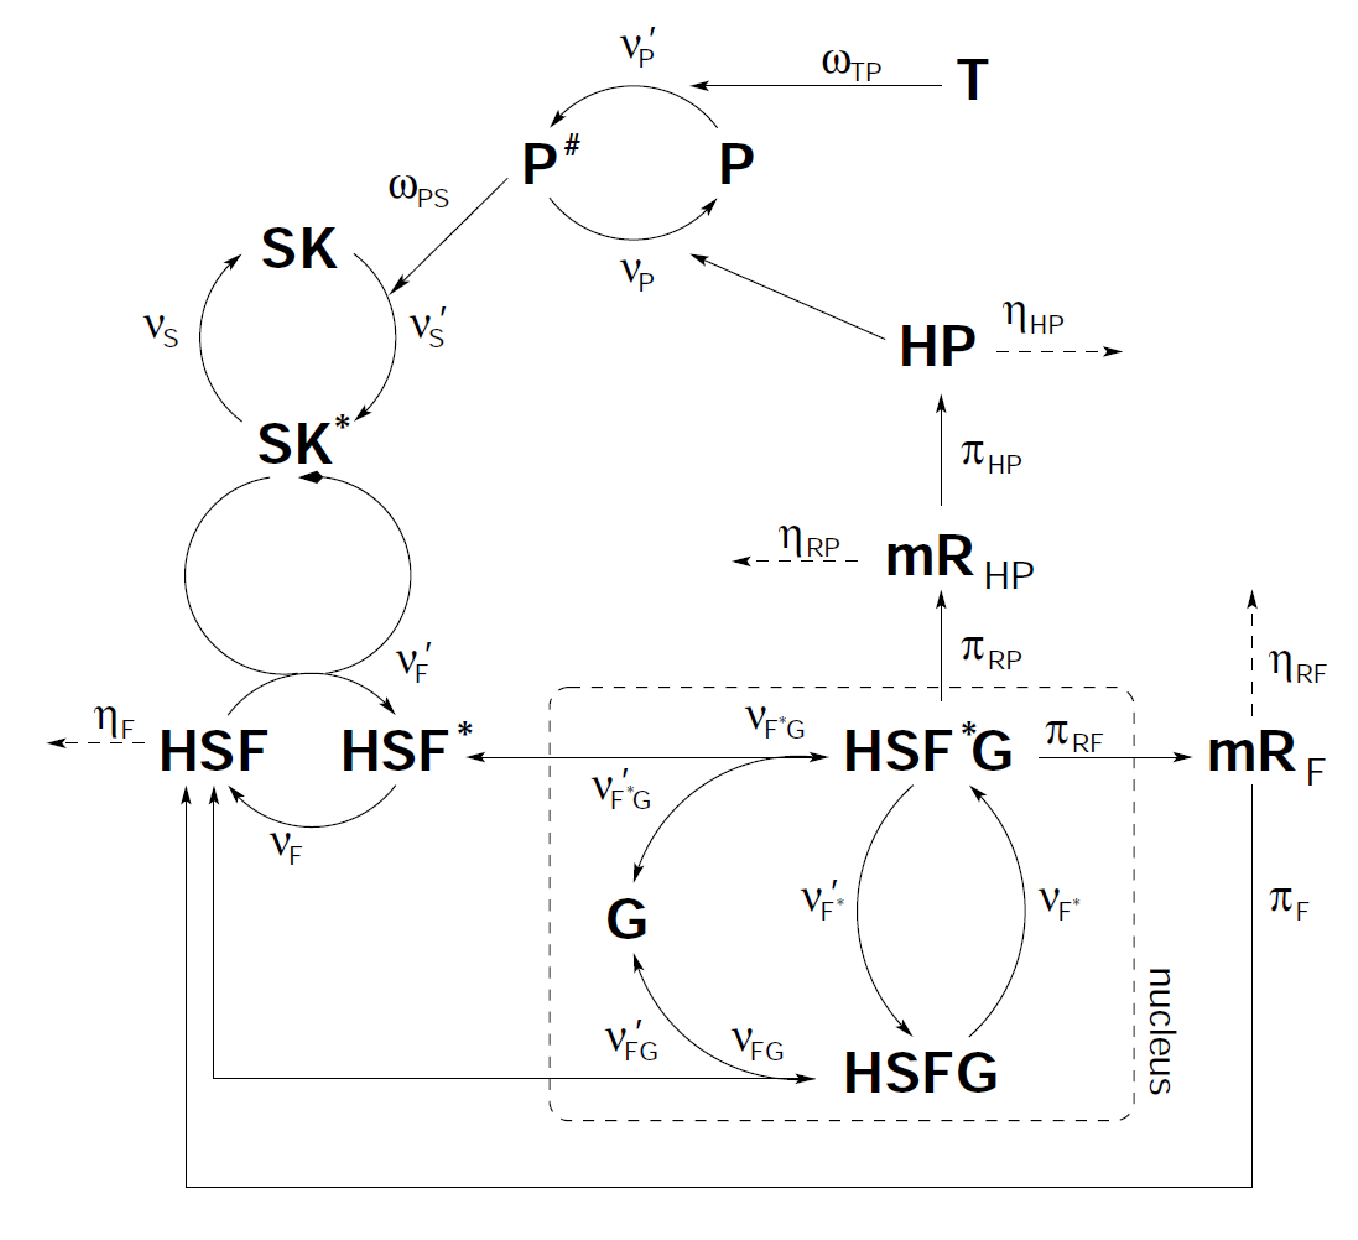
\includegraphics[width=\textwidth, height=0.40\textheight]{HSscheme.pdf}
%  }
%\endminipage\hfill
%\minipage{0.50\textwidth}
% \subfloat[The typical behavior of the model.\label{FigSimulationHSResponse}]{
%  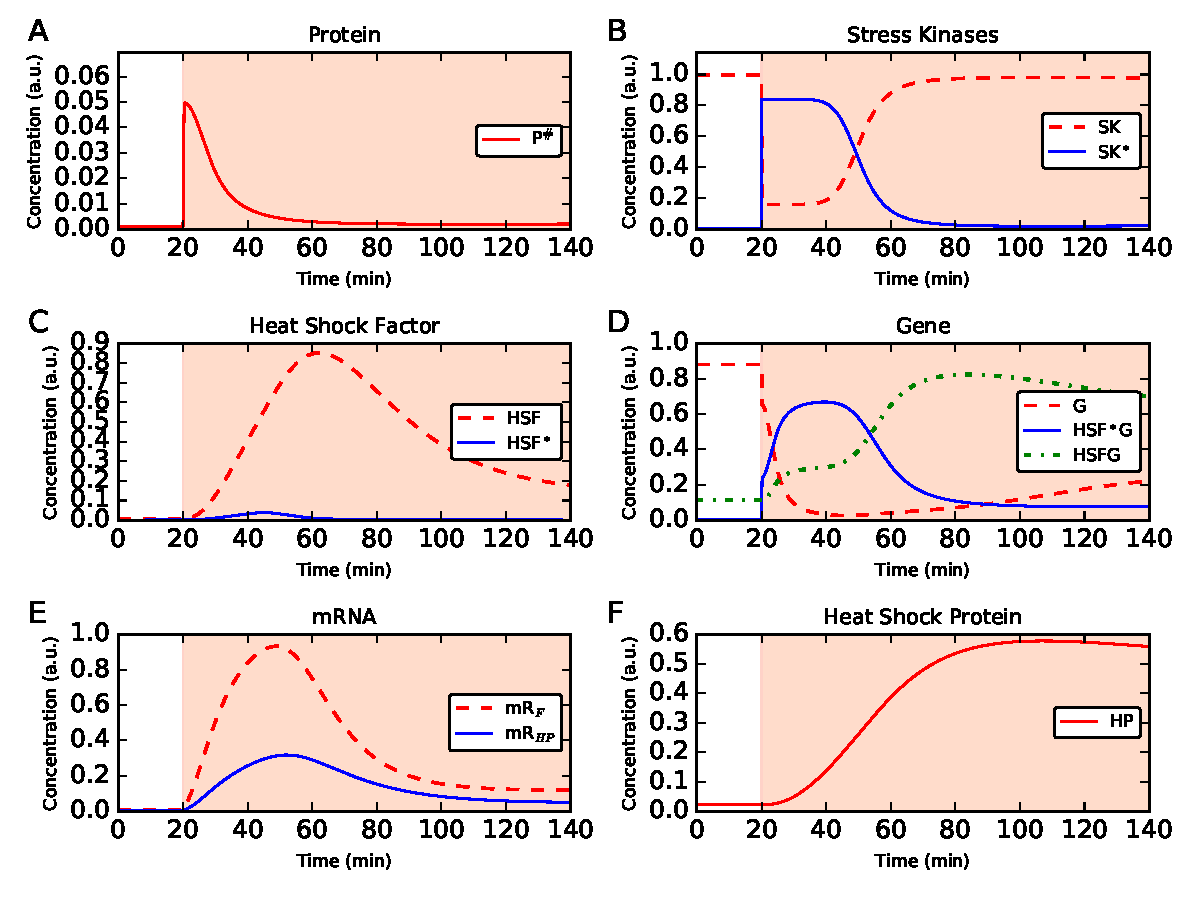
\includegraphics[width=\textwidth, height=0.40\textheight]{HeatShockResponse_SimulationHSResponse.pdf}
%  }
%\endminipage\hfill

\begin{figure*}
\centering
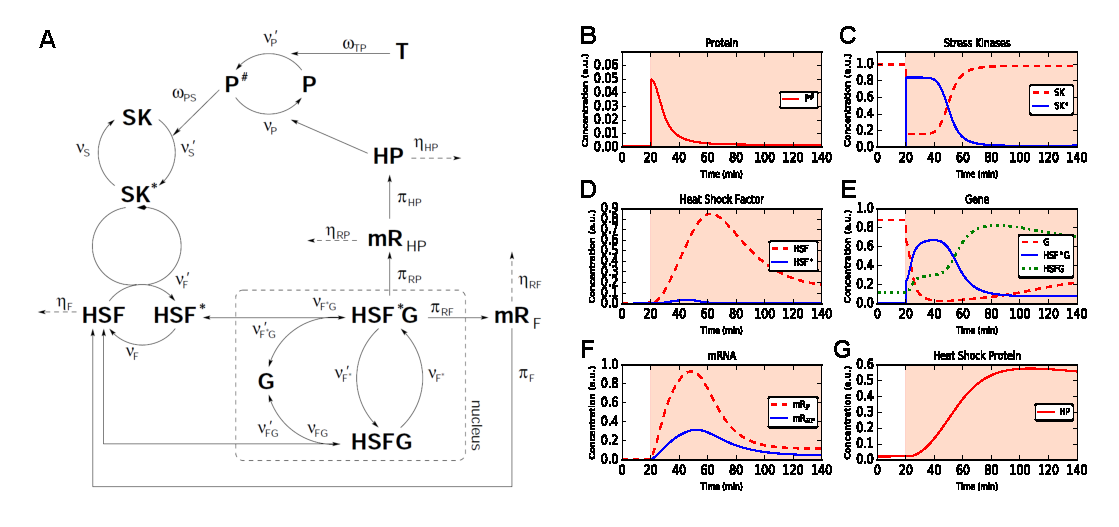
\includegraphics[width=\textwidth]{Figure1_Paper.pdf}
\caption{\small{\textbf{The dynamical model of the HSR.} \textbf{(A)} Scheme of the signalling network used to model the HSR. {This scheme is extracted from the experiments performed by Schmollinger et al.~\cite{Schmollinger2013} and inspired by the signaling mechanisms hypothesized in Fig.~11 therein, {to} which we add gene transcription and apply some simplifications as explained in the text. This signaling network represents the base to build our mathematical model of the HSR described in detail in Supplementary Material~\ref{Tables}.} Temperature T acts via %due to $\omega_\text{TP}$ 
the Arrhenius law $\omega_\text{TP}$ on the proteins P. 
Higher temperature increases $\nu_\text{P}'$ leading to more degenerated proteins P$^\#$. 
This activates stress kinases SK (SK* when active) by a {Hill kinetics} $\omega_\text{PS}$ which increases {phosphorylation} of the heat shock factor HSF (HSF* when active). 
If HSF* is bound to the gene G, mRNA for the heat shock factor HSF and for the heat shock protein HP is generated by the corresponding production rates $\pi$, respectively indicated by $mR_{HP}$ and $mR_{F}$. 
The mRNA is translated into the proteins HP and HSF and degraded by rates $\eta$. $HSF$*$G$ indicates $HSF$ active and bound to gene, $HSFG$ indicates $HSF$ inactive and bound to gene. \textbf{(B-G)} Typical behavior of the model illustrated inducing a HSR via an increase of the temperature from 25°C to 42°C applied at t = 20 min (represented by a red background in the figures). \textbf{(B)} Due to temperature increase at t = 20 min functional proteins P are mis-folded leading to an increased P$^\#$ level. \textbf{(C)} The degenerated proteins bring inactive stress kinases SK into their active form SK$^*$. \textbf{(D)} Due to active stress kinases, the heat shock factor (HSF) is phosphorylated (HSF$^*$). \textbf{(E)} The heat shock factor HSF binds to free gene loci G, the bound form HSF$^*$G activates mRNA production, and HSF un-binding blocks transcription. \textbf{(F)} The initiated gene transcription leads to mRNA production of the HSF and the heat shock protein as shown. \textbf{(G)} Due to translation of the corresponding mRNA, the HP concentration increases until the response is switched of. The small degeneration rate of the chaperon leads to a slow decrease after the onset of the HSR.
%Steady state concentrations before heat shock (at a constant temperature of 20°C) are [$P$] = 99.9 $m$M, [$P^\#$]=108 $\mu$M, [S]=105 $n$M, [$S^*$]=0.0108 $n$M, [$HSF$]=126 $n$M, [$HSF^*$]=0.0154 $n$M, [$G$]=2.18 $n$M, [$HSFG$]=15.0 $n$M, [$HSFG^*$]=0.000473 $n$M, [$mR_{F}$]=5.30 $n$M, [$mR_{HP}$]=5.23 $n$M and [$HP$]=25.5 $\mu$M.
The normalization factors used to represent the concentrations in arbitrary units can be found in Table \ref{TabRefVal} of the Supplementary Material.}}
  \label{Figure1label}
\end{figure*}

\clearpage

%\begin{figure*}
%%\minipage{0.30\textwidth}
%%  \includegraphics[width=\textwidth, height=0.20\textheight]%{FeedingExperimentVsDataALLinONE_RF_SimulationSTAUR2data.pdf}
  %\caption*{\small{Feeding with Staurosporine.}}
%%\endminipage\hfill
%%\minipage{0.30\textwidth}
%%  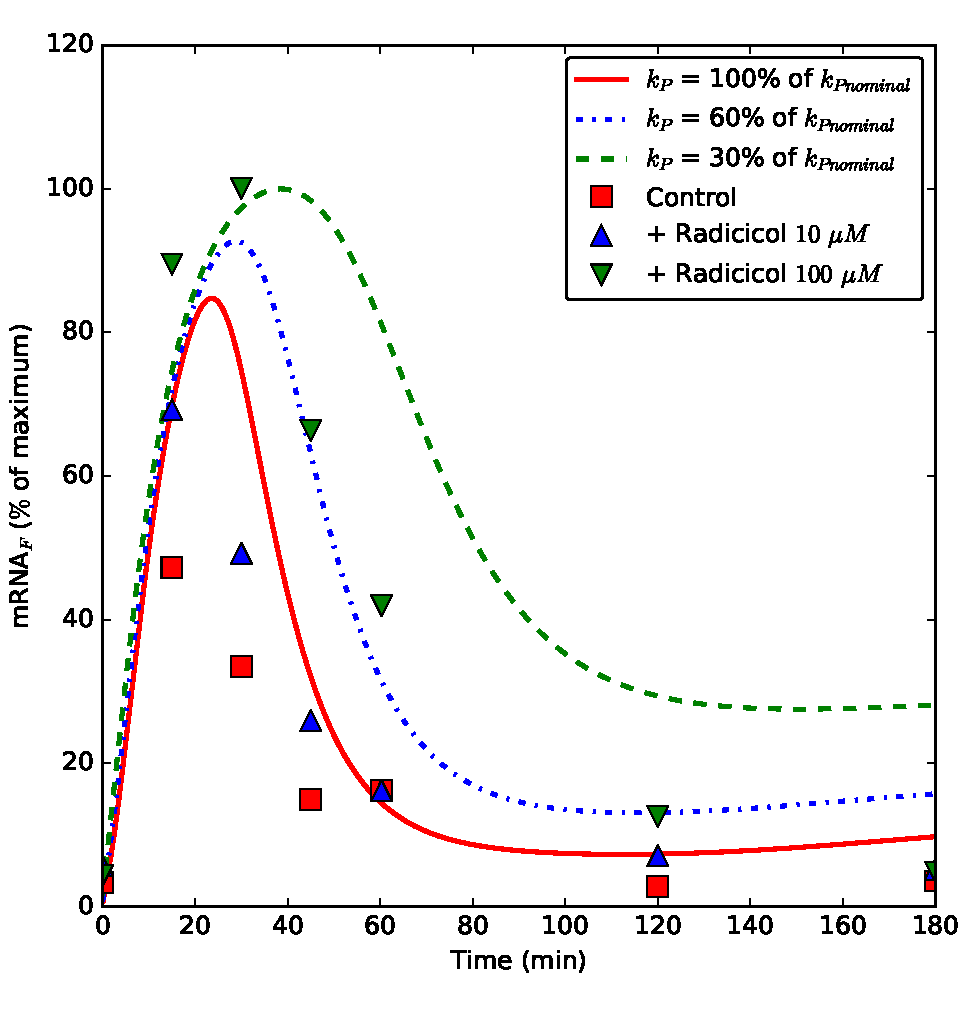
\includegraphics[width=\textwidth, height=0.20\textheight]{FeedingExperimentVsDataALLinONE_RF_SimulationRADdata.pdf}
%%  %\caption*{\small{Feeding with Radicicol.}}
%%\endminipage\hfill
%\minipage{1.00\textwidth}
%\hspace{-1.8cm}
% \subfloat[Monte Carlo scan of the parameter space, 1-dimensional projection.\label{Figure1}]{
%  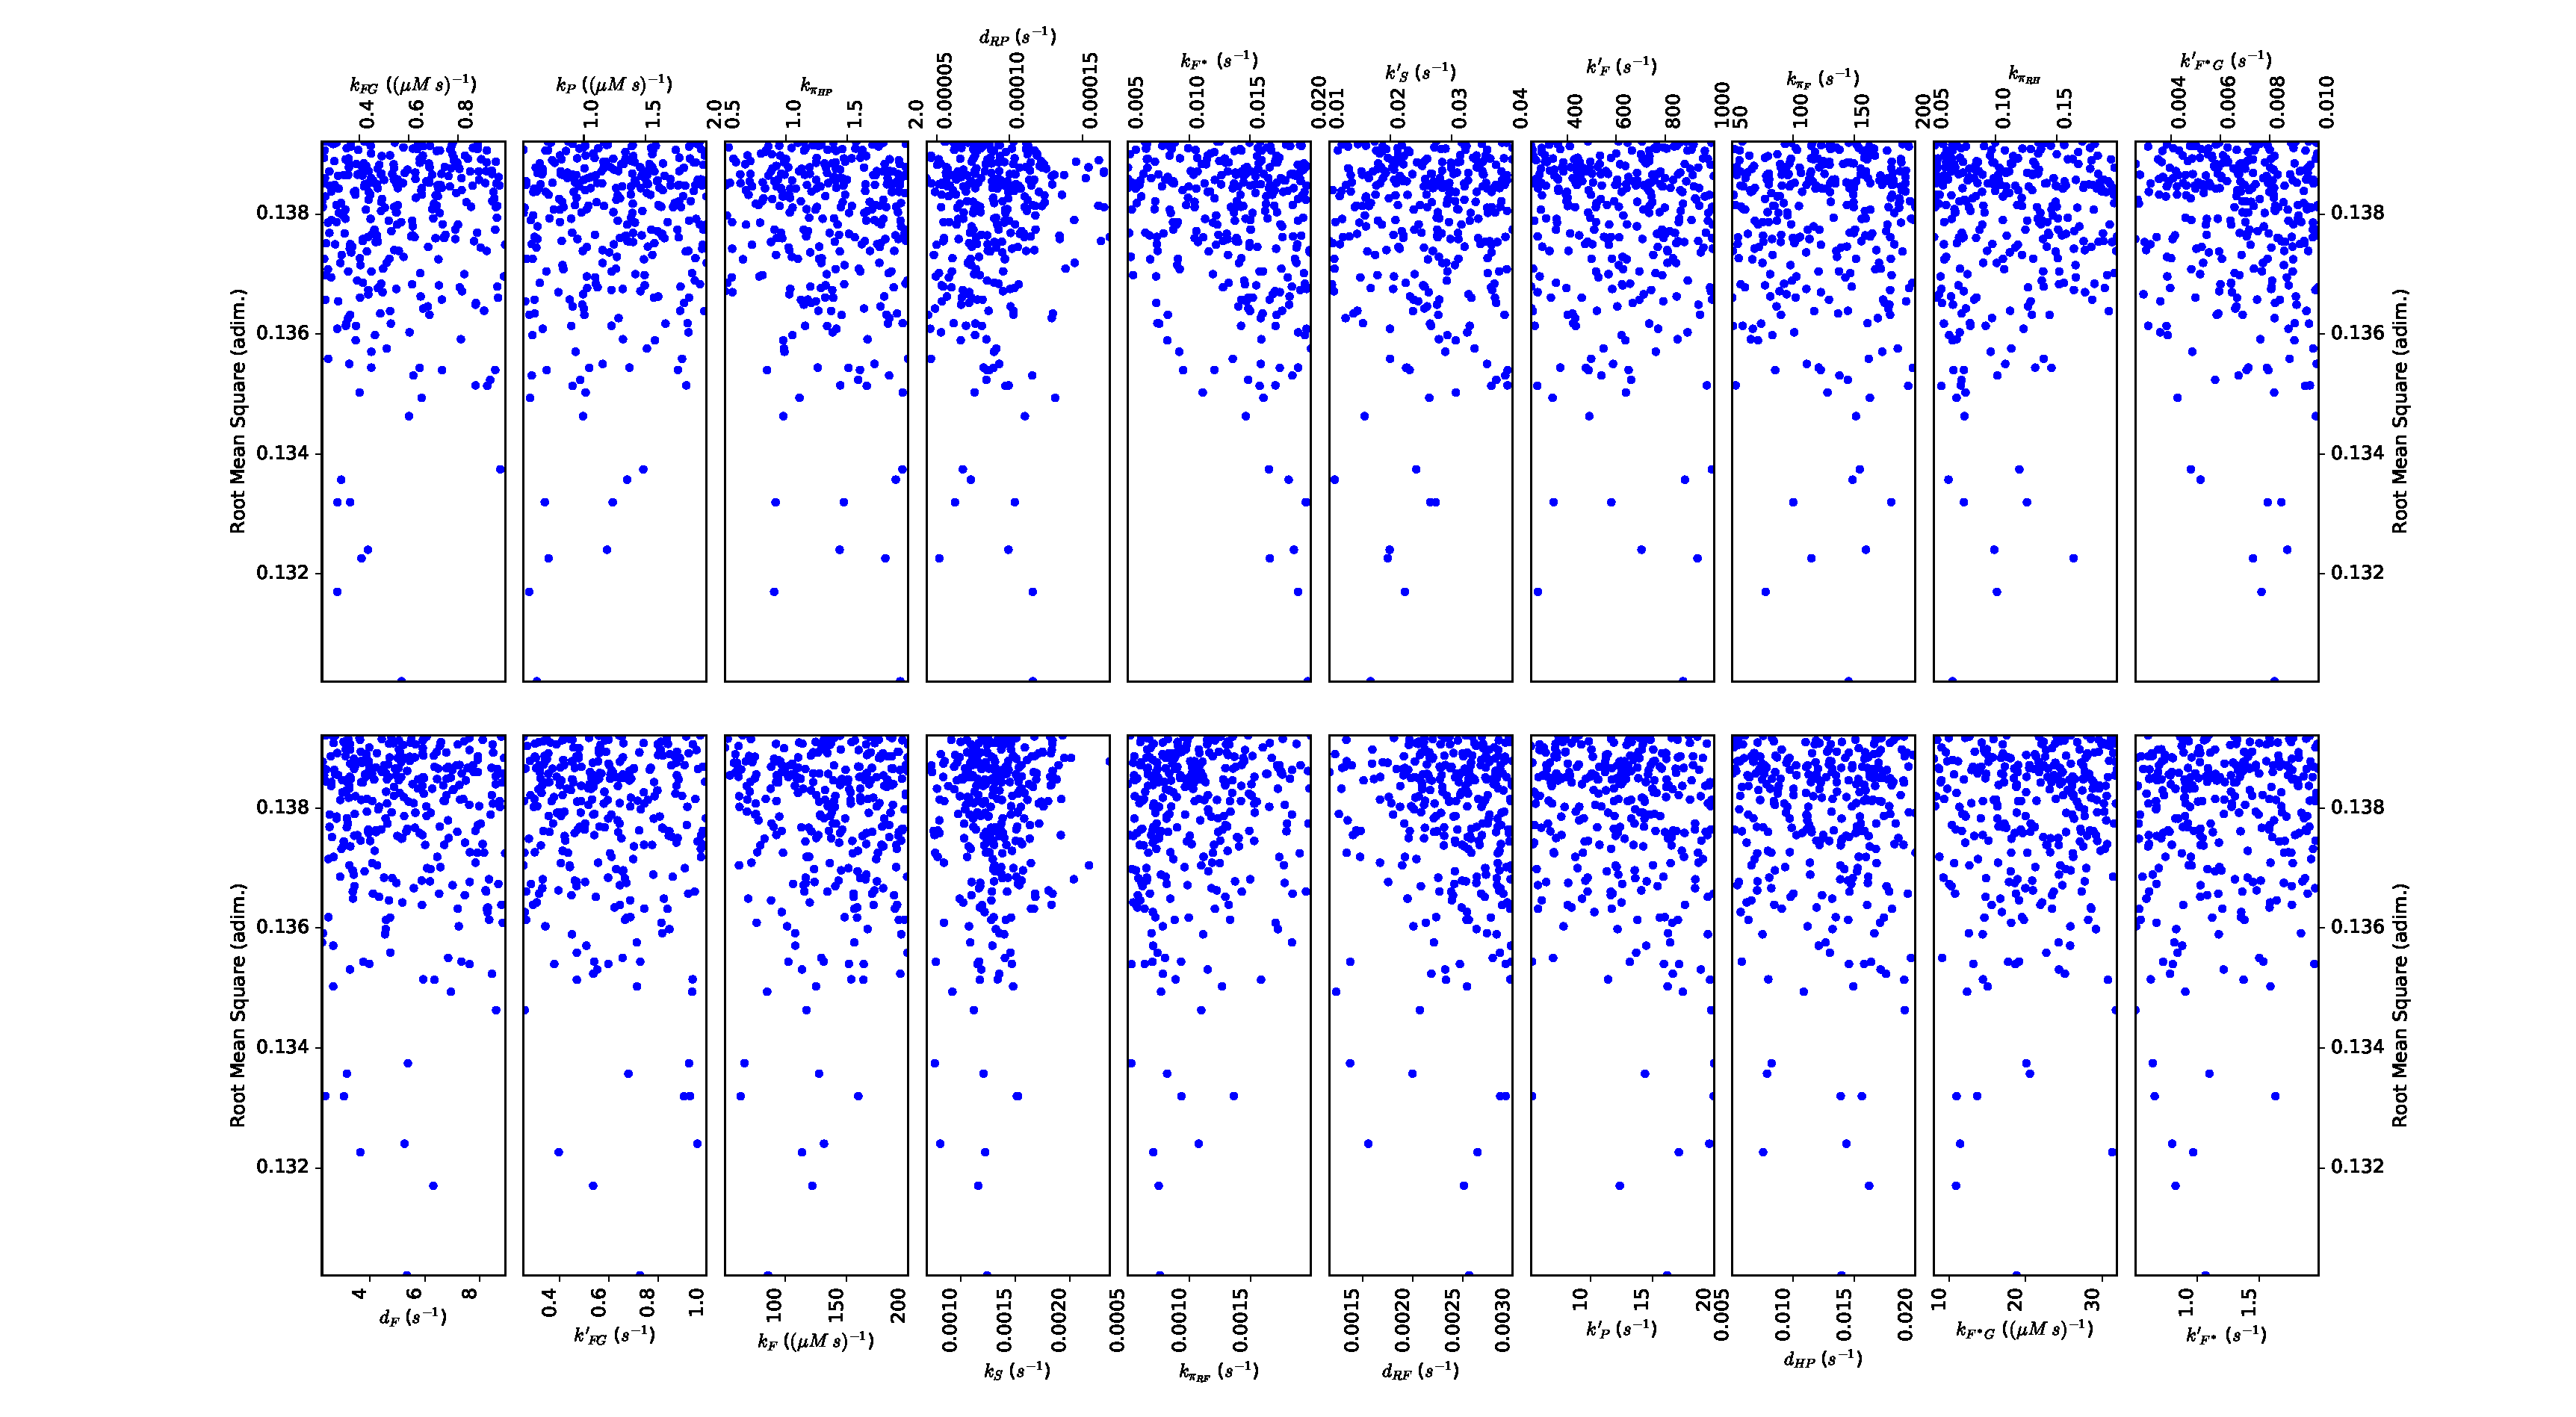
\includegraphics[ width=1.20\textwidth, height=0.35\textheight]{ScatterPlot20.pdf}
%  }%\caption*{\small{Monte Carlo scan of the parameter space.}}
%\endminipage\hfill
%%\minipage{1.00\textwidth}
%%\hspace{-1.8cm}
%% \subfloat[Monte Carlo scan of the parameter space, 2-dimensional projection.%\label{figure2}]{
%%  \includegraphics[ width=1.32\textwidth, height=0.52\textheight]{ScatterPlot400.pdf}
%%  }%\caption*{\small{Monte Carlo scan of the parameter space.}}
%%\endminipage\hfill
%\minipage{0.30\textwidth}
% \subfloat[Iterations of the gradient search.\label{GradientSearch_RMS}]{
%  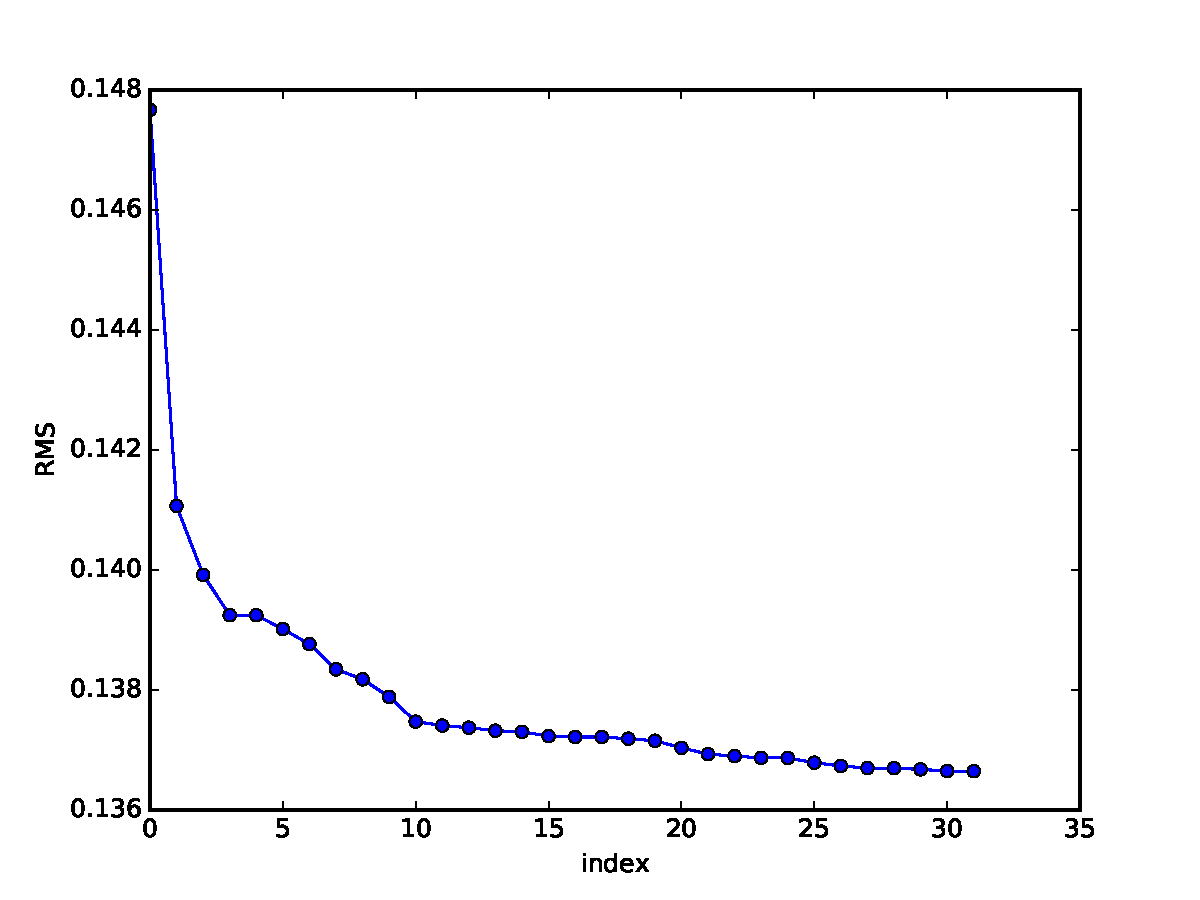
\includegraphics[width=\textwidth, height=0.27\textheight]{GradientSearch_RMS.pdf}
%  }%\caption*{\small{2C: Using the Gradient Search Algorithm.}}
%\endminipage\hfill
%\minipage{0.70\textwidth}
% \subfloat[Fitting to Controls of Feeding Experiments. Left HSF, right HSP.\label{2D}]{
%  \includegraphics[width=\textwidth, height=0.26\textheight]%{FittingToDataPAPERversionConrol.pdf}
%  }%\caption*{\small{2D: Fitting to Controls of Feeding Experiments. Left HSF, right %HSP.}}
%\endminipage\hfill
%\caption{\small{Calibration of the model. (a) 1-dimenasional projection w.r.t. each of %the 20 parameters of the Monte Carlo scan of the parameter space, for the points %corresponding to the 300 random parameter sets with lowest RMS. (b) RMS decrease for %subsequent iterations of the gradient search algorithm. (c) Data from the controls of %the feeding
%experiments of~\cite{Schmollinger2013}. These correspond to six curves
%representing the time evolution of the concentration of mRNA coding
%for HSF1 (left panel), and six curves for the mRNA coding for HSP90A (right panel), %under heat
%shock and no inhibitor treatment. The superposed continuous black line show the model %prediction obtained with the final parameter set.}}
%  \label{Figure2label}
%\end{figure*}
%% (b) 2-dimensional projection w.r.t. each couple of parameters of the Monte Carlo scan %of the parameter space, showing RMS (colours) for the same points of Fig.~\ref{Figure1}. 

\begin{figure*}
\centering
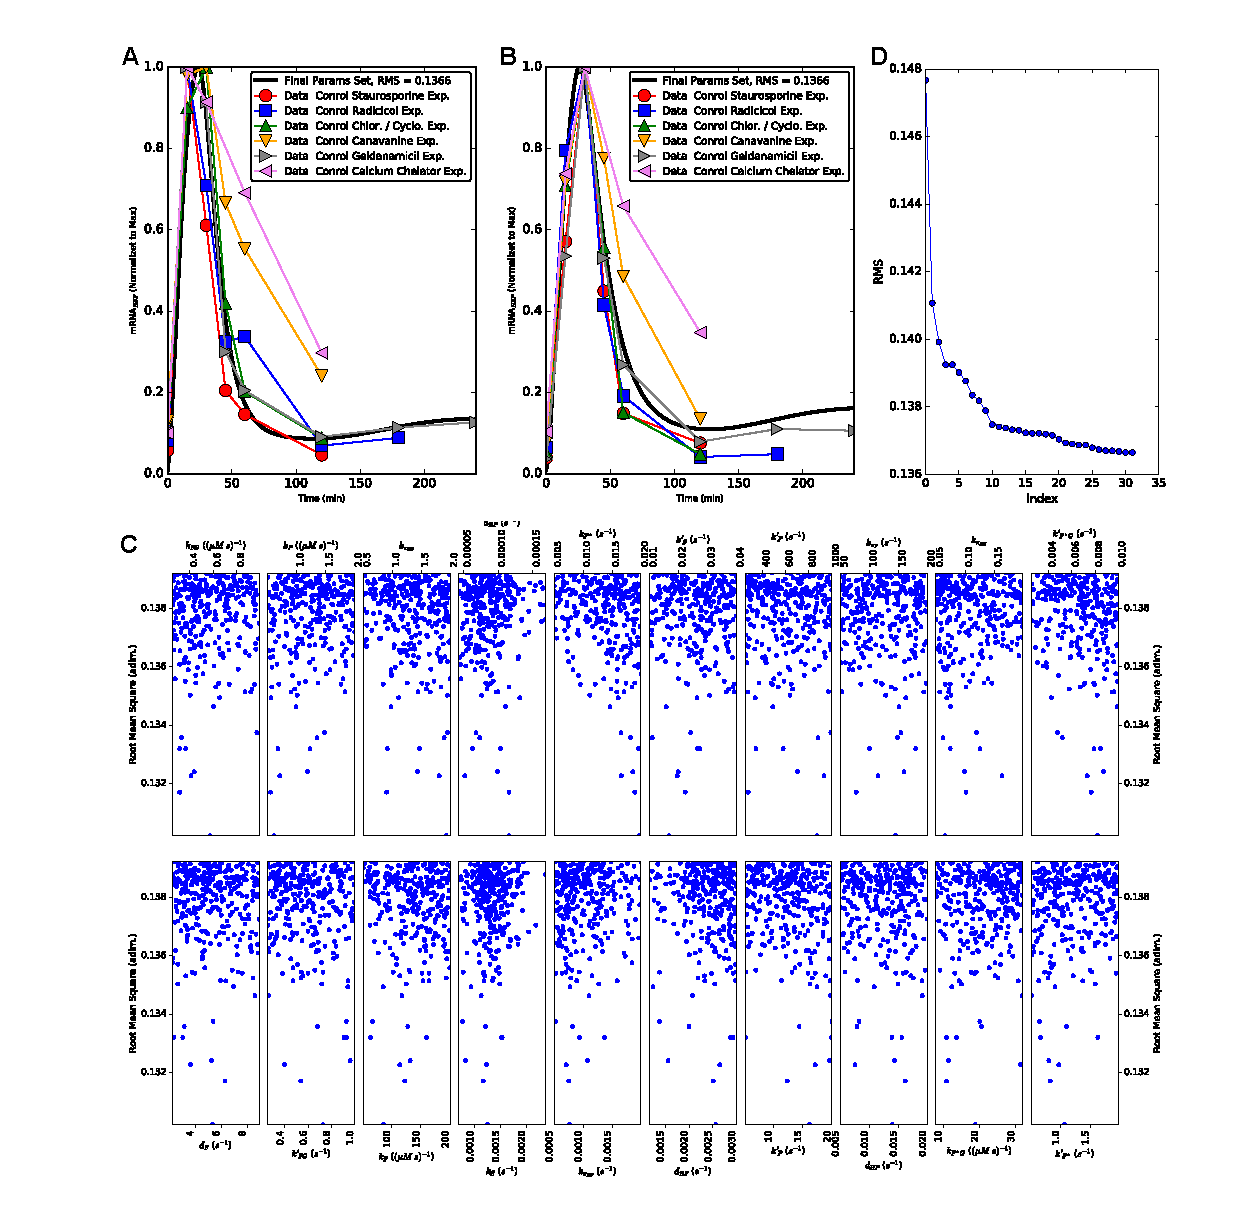
\includegraphics[width=\textwidth]{Figure2_Paper.pdf}
\caption{\small{\textbf{Model parameterization.} \textbf{(A,B)} Data from the controls of the feeding
experiments of Schmollinger et al.~\cite{Schmollinger2013}. These correspond to six curves
representing the time evolution of the concentration of mRNA coding
for HSF1 \textbf{(A)}, and six curves for the mRNA coding for HSP90A \textbf{(B)}, under heat
shock and no inhibitor treatment. The superposed continuous black line shows the model prediction obtained with the final parameter set. \textbf{(C)} Projection w.r.t. each of the 20 parameters of the Monte Carlo (MC) scan of the parameter space, for the points corresponding to the 300 random parameter sets with lowest RMS {among the $10^5$ sets randomly generated. The RMS corresponding to these $10^5$ sets ranged between 0.130 and 0.700, while this panel is strongly magnified and only shows parameter sets with RMS between 0.130 and 0.139. The vertical red line in each sub-panel indicates the fiducial value of the corresponding parameter, i.e. the starting point of the two alternative calibration approaches used, the MC described in this panel, and the gradient search eventually employed. The yellow star in each sub-panel indicates the parameter values finally retained after the gradient search, referred to as the "final parameter set" (Supplementary Material Table~\ref{TabKs}). These values are relatively close to the fiducial values, and the corresponding RMS of 0.137 is close to the lower extreme of the range of values obtained with the MC (0.130 to 0.700).} \textbf{(D)}} RMS decrease for subsequent iterations of the gradient search algorithm.}
\label{Figure2label}
\end{figure*}

\clearpage

%\begin{figure*}
%\minipage{0.50\textwidth}
% \subfloat[Feeding with Staurosporine.\label{FigStaurSim}]{
%  \includegraphics[width=\textwidth, height=0.30\textheight]%{FeedingExperimentVsDataALLinONE_RF_SimulationSTAUR2data.pdf}
%  }%\caption*{\small{Feeding with Staurosporine.}}
%\endminipage\hfill
%\minipage{0.50\textwidth}
% \subfloat[Feeding with Radicicol.\label{FigRadSim}]{
%  \includegraphics[width=\textwidth, height=0.30\textheight]%{FeedingExperimentVsDataALLinONE_RF_SimulationRADdata.pdf}
%  }%\caption*{\small{Feeling with Radicicol.}}
%\endminipage\hfill
%\minipage{0.50\textwidth}
% \subfloat[Double Heat Shock.\label{ARS2}]{
%  \includegraphics[width=\textwidth, height=0.30\textheight]%{HeatShockARSExpDoubleHS_SimulationARSdoubleHSshort.pdf}
%  }%\caption*{\small{
%  %Simulating double heat shock experiment and comparison with the corresponding data %from \cite{Schroda2000}.Double Heat Shock.}}
%\endminipage\hfill
%\minipage{0.50\textwidth}
% \subfloat[HP expression.\label{FigTimeCoruseData}]{
%  \includegraphics[width=\textwidth, height=0.30\textheight]%{TimeCoruseData_SimulationHSResponseVsData.pdf}
%  }%\caption*{\small{Feeding with Staurosporine.}}
%\endminipage\hfill
%\minipage{0.50\textwidth}
%  \includegraphics[width=\textwidth, height=0.32\textheight]%{HeatShockResponse_SimulationDoubleHeat30min.pdf}
%  \caption*{\small{Second heat shock after 30 minutes.}}
%\endminipage\hfill
%\minipage{0.50\textwidth}
%  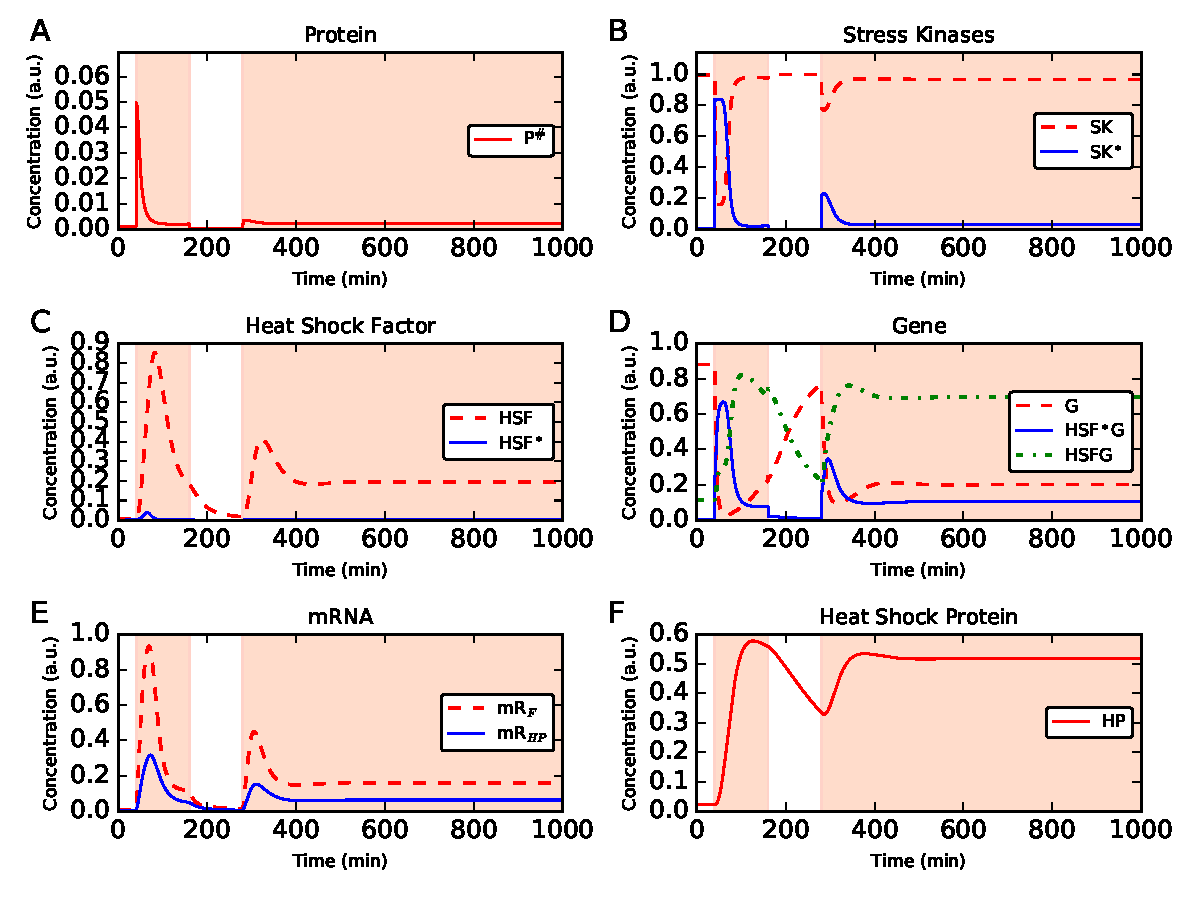
\includegraphics[width=\textwidth, height=0.32\textheight]{HeatShockResponse_SimulationDoubleHeat2h.pdf}
%  \caption*{\small{Second heat shock after 2 hours.}}
%\endminipage\hfill
%\minipage{0.50\textwidth}
%  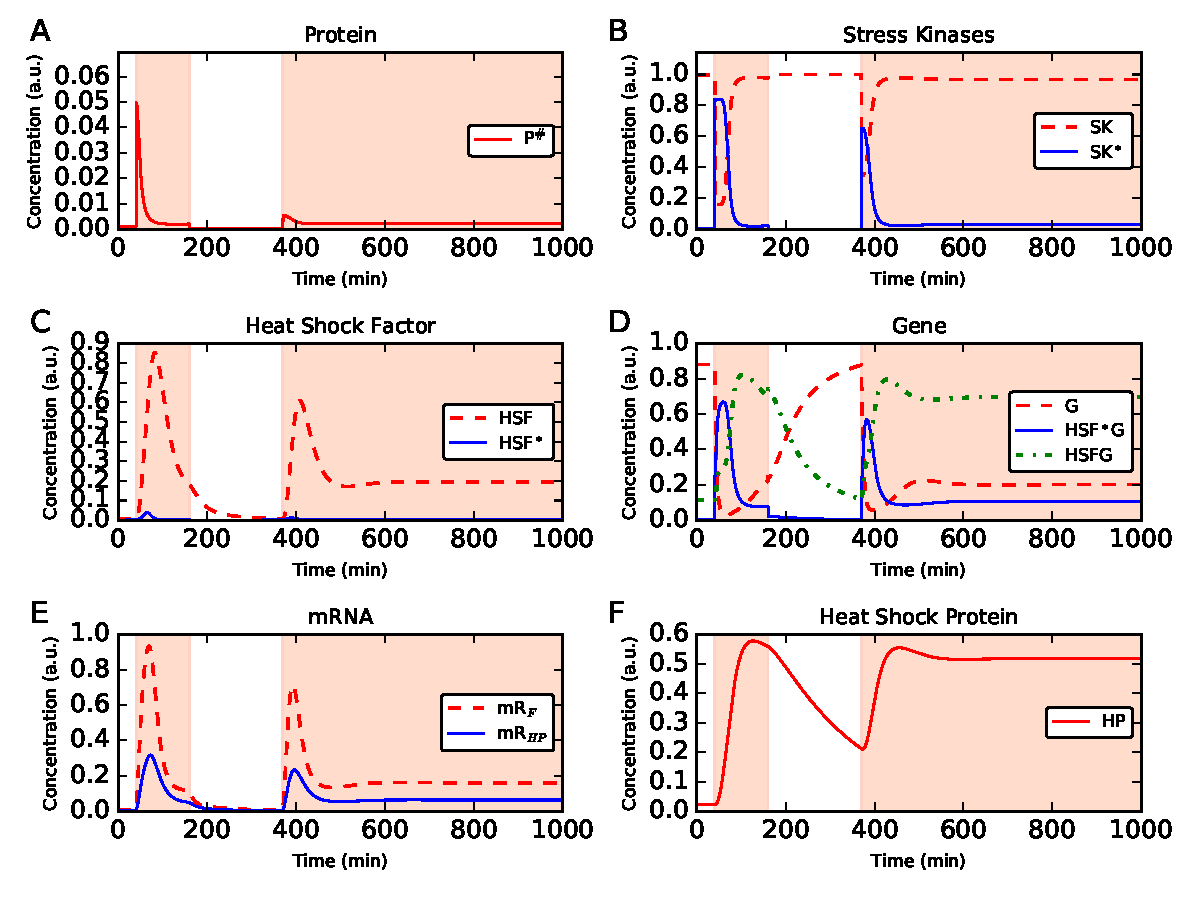
\includegraphics[width=\textwidth, height=0.32\textheight]{HeatShockResponse_SimulationDoubleHeat3h30min.pdf}
%  \caption*{\small{Second heat shock after 3 hours and 30 minutes.}}
%\endminipage\hfill
%\minipage{0.50\textwidth}
%  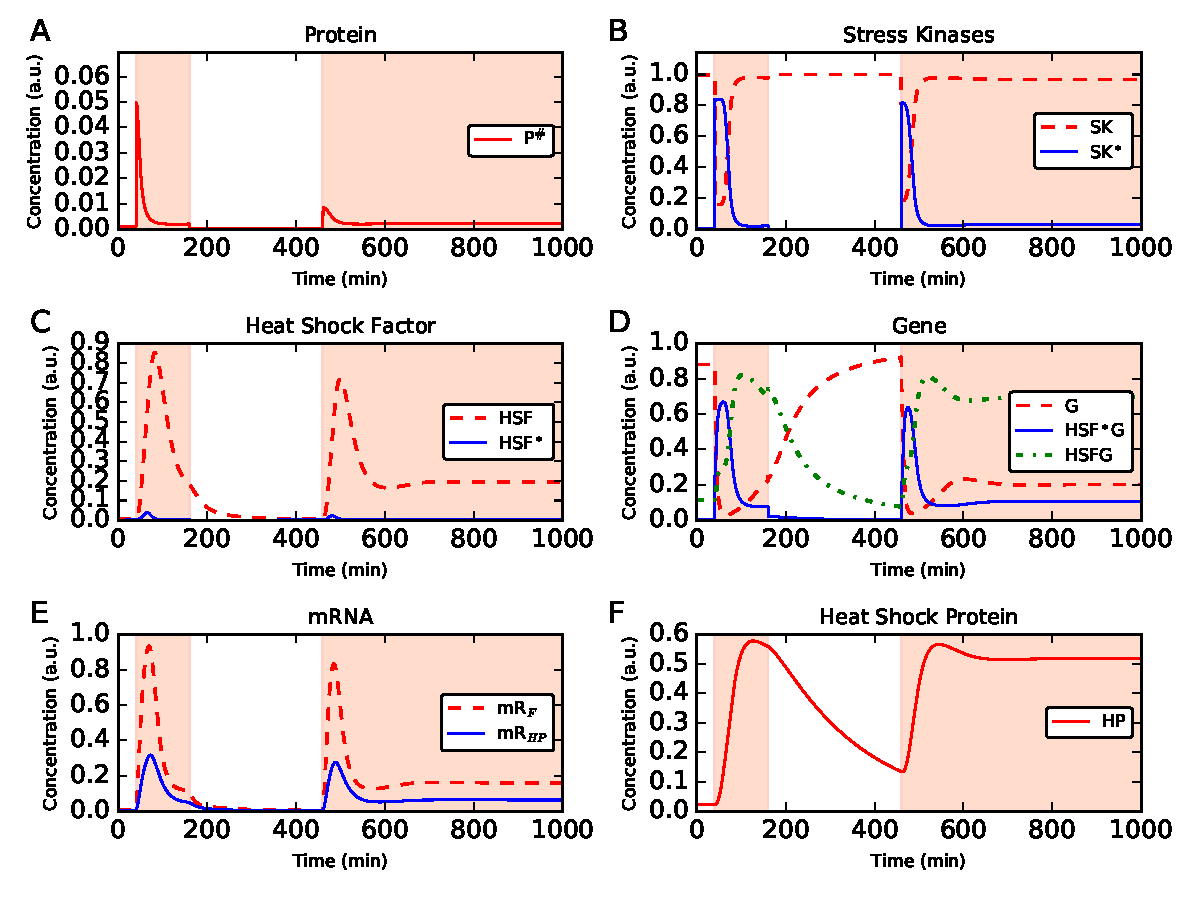
\includegraphics[width=\textwidth, height=0.32\textheight]{HeatShockResponse_SimulationDoubleHeat5h.pdf}
%  \caption*{\small{Second heat shock after 5 hours.}}
%\endminipage\hfill
%\caption{\small{Model validation comparing model predictions with data from feeding experiments of \cite{Schmollinger2013} using Staurosporine (a) and Radicicol (b), and double HS experiments (c) Simulating the double heat shock experiment and comparison with the corresponding data from \cite{Schroda2000}. We see that a full HSR is possible only about $5$ h after the first HS. (d) Comparison between the model predictions for the variation of the concentration of HP under HS and the corresponding data from \cite{Muehlhaus2011}. The scale on the left side refers to the simulation results, the scale on the right side to the data. An exact correspondence of one scale into the other is not possible since we lack the necessary information.}}
%  \label{{Figure3label}}
%\end{figure*}
%\clearpage

\begin{figure*}
\centering
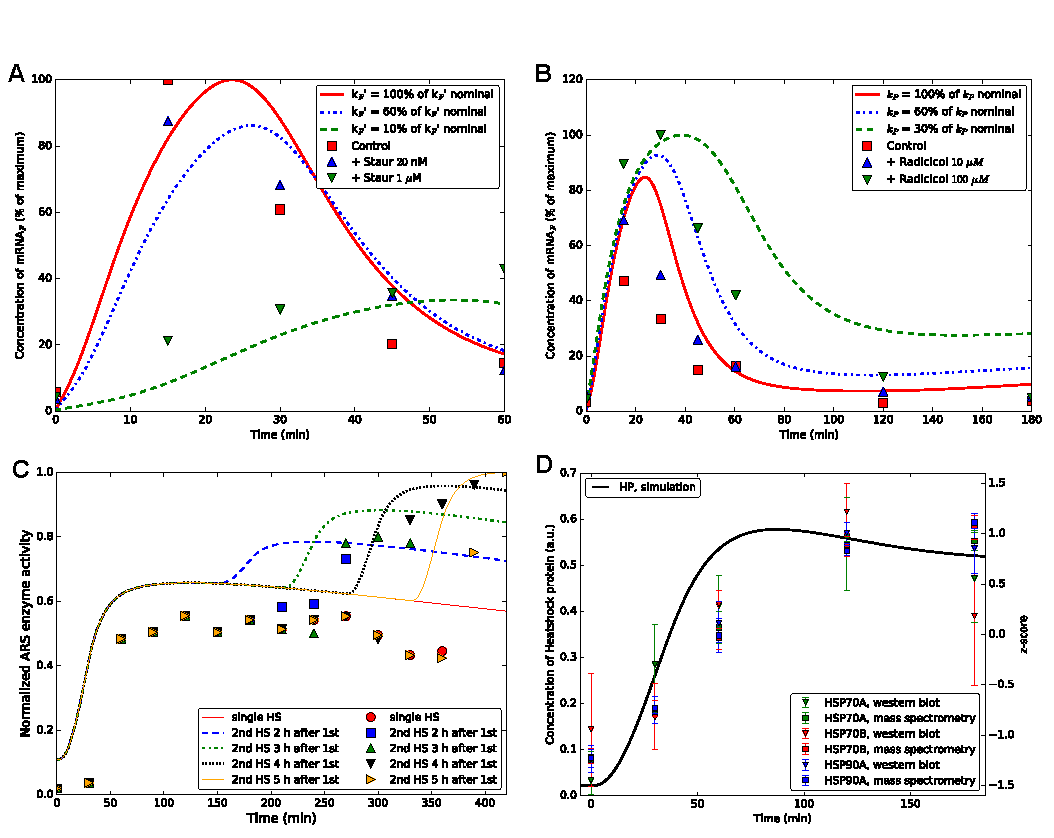
\includegraphics[width=\textwidth]{Figure3_Paper.pdf}
\caption{\small{\textbf{Comparisons between model predictions and data.} Feeding experiments by Schmollinger et al.~\cite{Schmollinger2013} using Staurosporine \textbf{(A)} and Radicicol \textbf{(B)}. \textbf{(C)} Simulating the double HS experiment and comparison with the corresponding data from Schroda et al.~\cite{Schroda2000}. {As in that experimental study, two HSs of 30 minutes duration each were applied to our model at a distance of 2, 3, 4, and 5 hours (blue, green, black and yellow curve respectively), and compared to the response to only one HS of 30 minutes duration (red curve).} We see that a full HSR{, i.e. a HSR in which the increase in the concentration of $HSP$ (and thus in the ARS enzyme activity) has approximately the same magnitude for the second HS as for the first HS,} is possible only when the second HS occurs at least $5$ h after the first HS. \textbf{(D)} Comparison between the model predictions for the variation of the concentration of HP under HS and the corresponding data from M\"uhlhaus et al. \cite{Muehlhaus2011}. The scale on the left side refers to the simulation results, the scale on the right side to the data. An exact correspondence of one scale into the other is not possible since we lack the necessary information.}
}
\label{Figure3label}
\end{figure*}

\clearpage

%\begin{figure*}
%\minipage{1.00\textwidth}
% \subfloat[Simulated response to natural daily temperature variation.\label{24hsin}]{
%  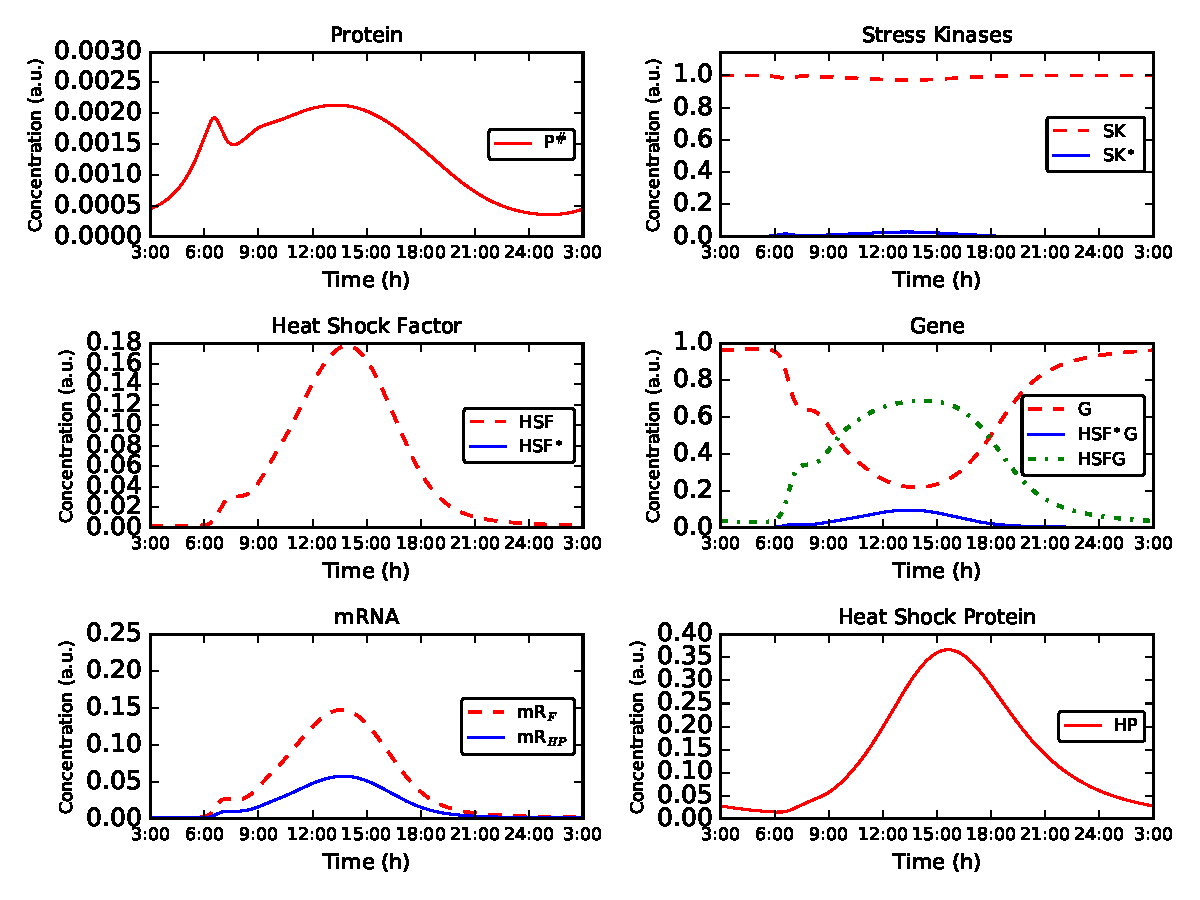
\includegraphics[width=\textwidth, height=0.45\textheight]{HeatShockResponse_SimulationWEIRDTsin.pdf}
%  }%\caption*{\small{simulation of the response of the system to a temperature variation reproducing that of a hot day.}}
%\endminipage\hfill
%\minipage{0.30\textwidth}
% \subfloat[Natural temperature variation.\label{Temperature24hsin}]{
%  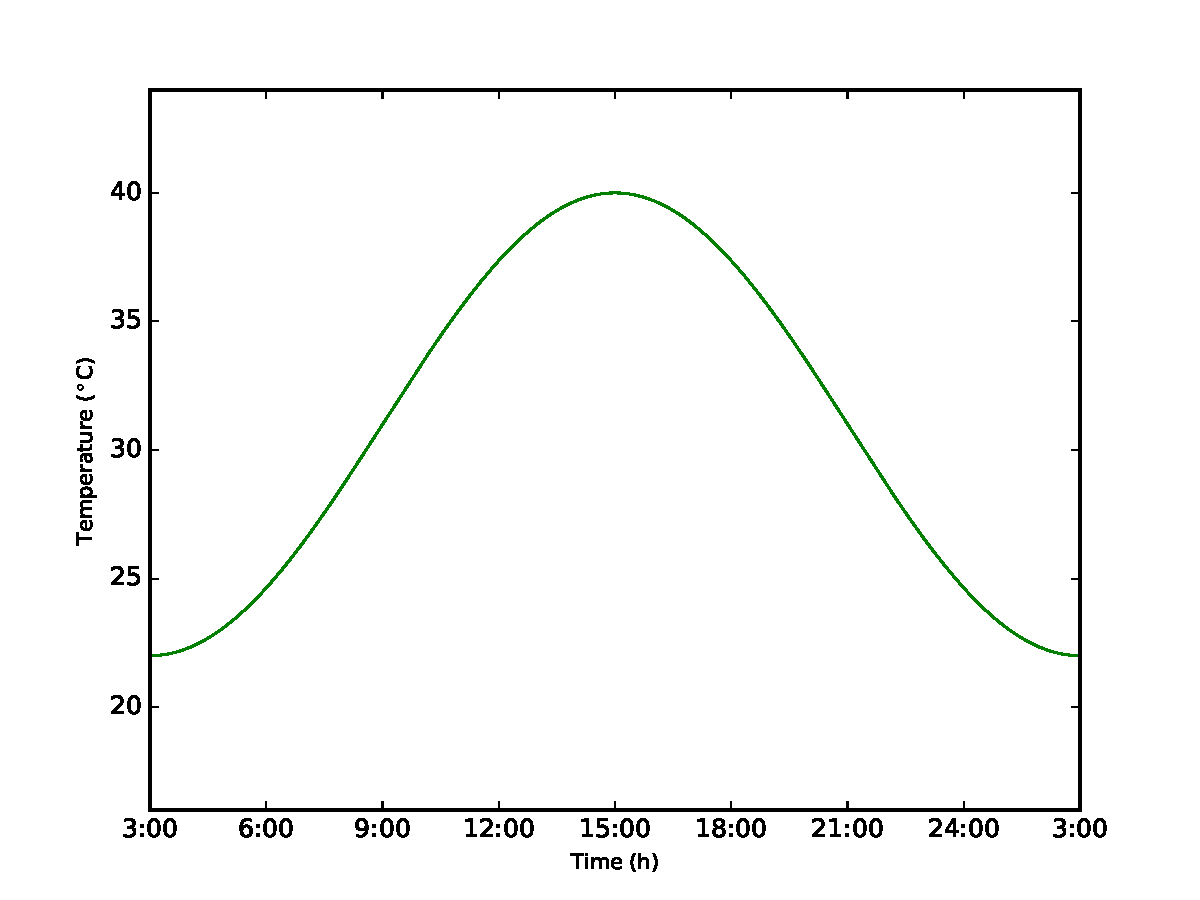
\includegraphics[width=\textwidth, height=0.20\textheight]{Temperature_SimulationWEIRDTsin.pdf}
%  }%\caption*{\small{Temperature variation reproducing that of a hot day.}}
%\endminipage\hfill
%\minipage{0.30\textwidth}
% \subfloat[Considering increasing periods.\label{4C}]{
%  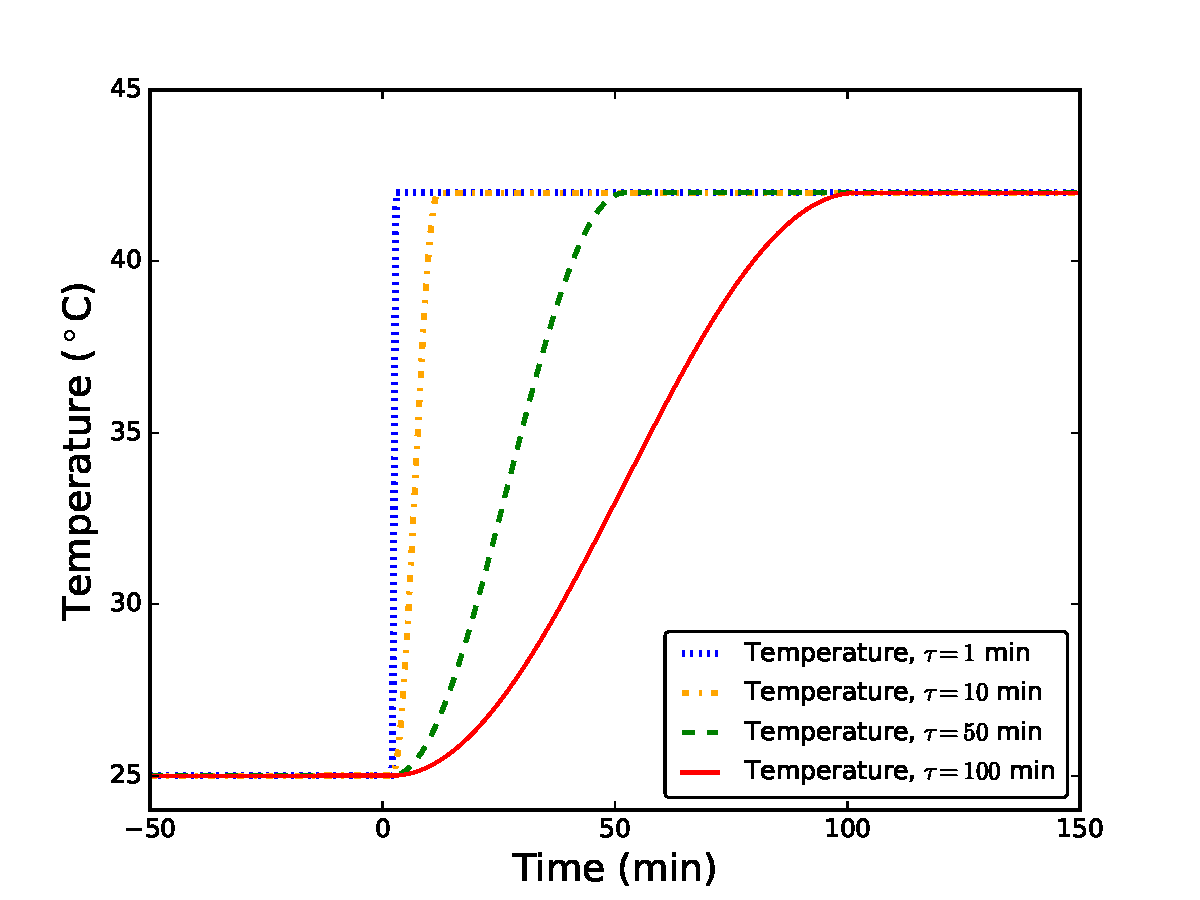
\includegraphics[width=\textwidth, height=0.20\textheight]{TemperatureManyTaus.pdf}
%  }%\caption*{\small{Temperature variation reproducing that of a hot day.}}
%\endminipage\hfill
%\minipage{0.40\textwidth}
% \subfloat[Maximum accumulated unfolded proteins.\label{UnfoldedPfuncOfTau}]{
%  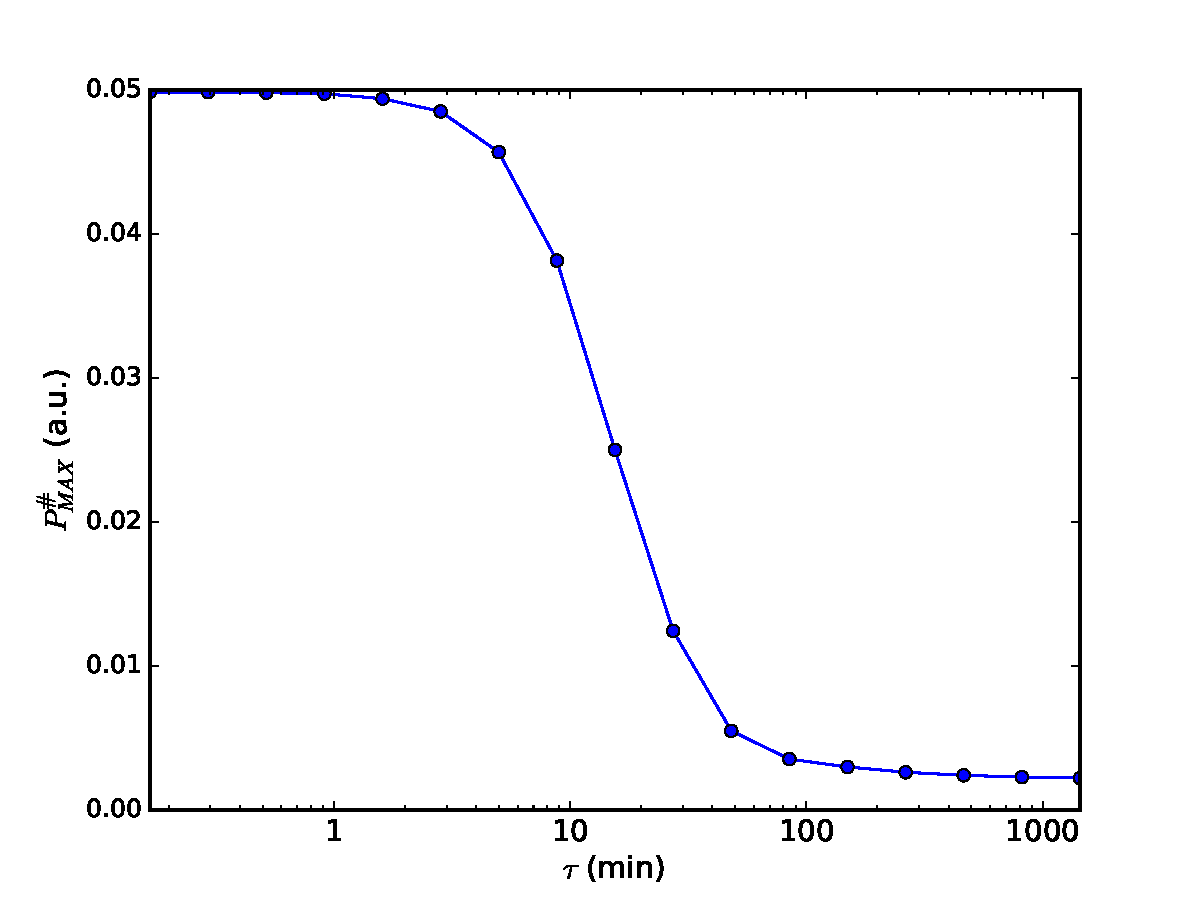
\includegraphics[width=\textwidth, height=0.20\textheight]{UnfoldedPfuncOfTau.pdf}
%  }%\caption*{\small{Maximum of accumulated unfolded proteins.}}
%\endminipage\hfill
%\caption{\small{HSR is adapted to natural daily temperature variation. (a) Simulation of the response of the system to a temperature variation reproducing that of a hot day (shown in Fig.~\ref{Temperature24hsin}). The concentration of unfolded proteins is kept very low, well below one percent of the total amount of proteins $\left[P\right]+\left[P^\#\right]$ (panel A, where you can notice that the vertical scale is magnified w.r.t. the same panel of the previous figures). (b) Temperature variation reproducing that of a hot day, used as input for the simulation of Fig.~\ref{24hsin}. (c) Considering increasing priods of time to increase temperature from a lower to a higher value. (d) Study of how the maximum concentration of unfolded proteins accumulated at steady state during a HS depends on how fast the temperature has increased from the initial (lower) value to the final (higher) value.}}
%  \label{{Figure4label}}
%\end{figure*}

\begin{figure*}
\centering
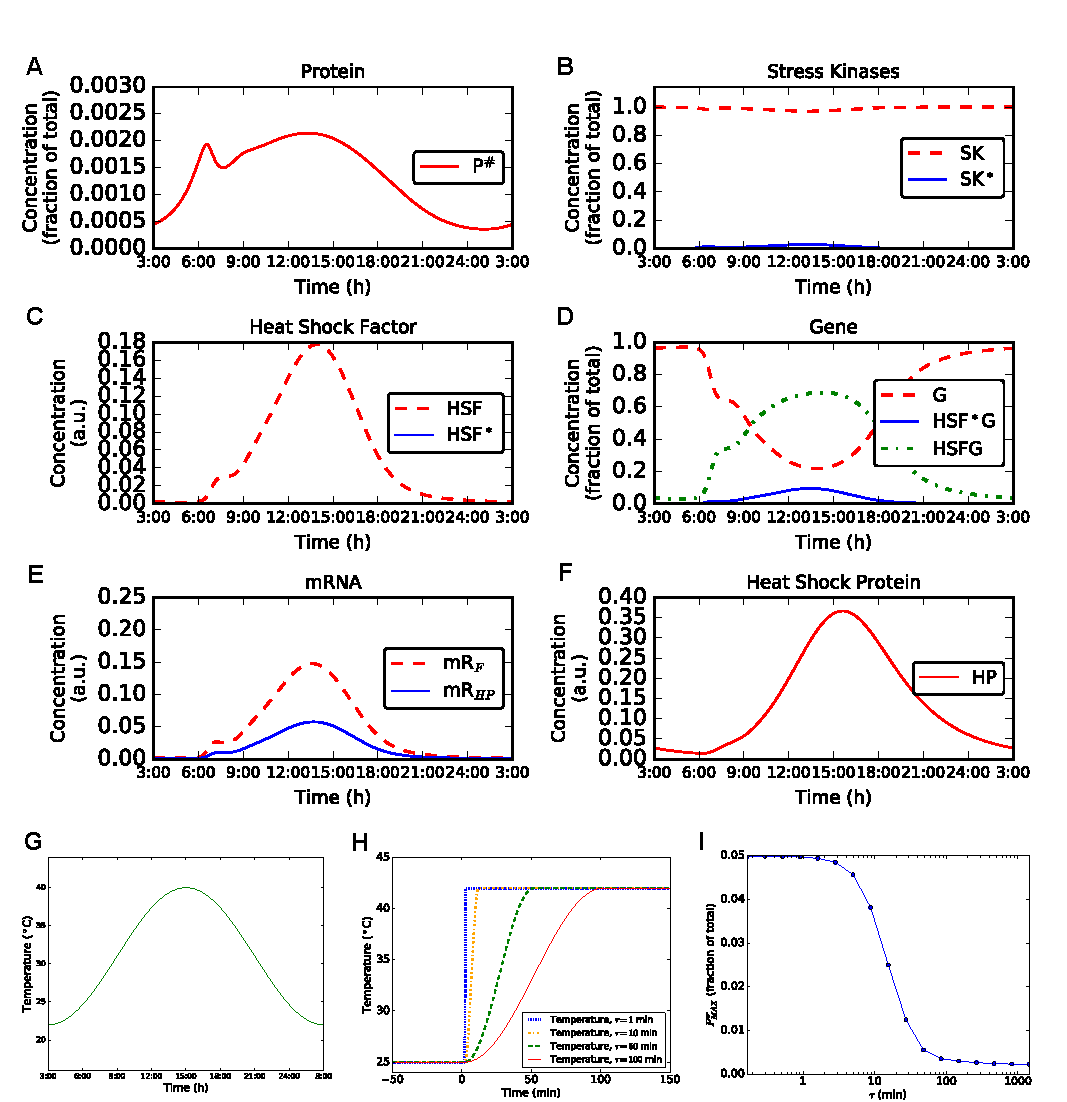
\includegraphics[width=\textwidth]{Figure4_Paper.pdf}
\caption{\small{\textbf{HSR is {tailored to handle} natural daily temperature variation.} \textbf{(A-F)} Simulation of the response of the system to a temperature {fluctuation approximating a typical hot day}, shown in \textbf{(G)}. The concentration of unfolded proteins is kept very low, well below one percent of the total amount of proteins $\left[P\right]+\left[P^\#\right]$ (note the different vertical scale in panel (A), compared to previous figures). {\textbf{(H)} We further consider temperature variations from $25^\circ\text{C}$ to $42^\circ\text{C}$ occurring across increasing periods of time, here shown from $1$ to $100$ minutes. \textbf{(I)} Study of how the maximum concentration of unfolded proteins accumulated at steady state during a HS depends on how fast the temperature has increased from the initial (lower) value to the final (higher) value, considering times from $10^{-1}$ to $10^{3}$ minutes.}}
}
\label{Figure4label}
\end{figure*}

\end{document}
